\PassOptionsToPackage{unicode}{hyperref}
\documentclass[aspectratio=1610, professionalfonts, 9pt]{beamer}

\usefonttheme[onlymath]{serif}
\usetheme[showtotalframes]{tudo}


\usepackage{polyglossia}
\setmainlanguage{english}

% Mathematik
\usepackage{mathtools}

% Enable Unicode-Math and follow the ISO-Standards for typesetting math
\usepackage[
  math-style=ISO,
  bold-style=ISO,
  sans-style=italic,
  nabla=upright,
  partial=upright,
]{unicode-math}
\setmathfont{Latin Modern Math}

% nice, small fracs for the text with \sfrac{}{}
\usepackage{xfrac}

\usepackage{multicol}
\usepackage{graphicx}
\usepackage{amssymb}
\usepackage{amsmath}
\usepackage{xparse}
\usepackage{braket}
\usepackage{units}
\usepackage[locale=DE,separate-uncertainty=true,per-mode=reciprocal,output-decimal-marker={,},]{siunitx}
\sisetup{
  round-mode          = places, % Rounds numbers
  round-precision     = 2, % to 2 places
}
\usepackage[section]{placeins}
\usepackage{pdflscape}
\usepackage{expl3}
\usepackage{bookmark}
\usepackage{booktabs}
%Komma als Dezimaltrenner in der mathe Umgebung, um in Umgebungen wie [0, 2] ein Leerzeichen nach dem Komma zu erhalten einfach eins setzen
\usepackage{icomma}
\usepackage{cancel}

\usepackage[
  backend=biber,   % use modern biber backend
  autolang=hyphen, % load hyphenation rules for if language of bibentry is not
                   % german, has to be loaded with \setotherlanguages
                   % in the references.bib use langid={en} for english sources
]{biblatex}
\addbibresource{references.bib}  % die Bibliographie einbinden
\DefineBibliographyStrings{german}{andothers = {{et\,al\adddot}}}



\usepackage{hyperref}
\usepackage{subfigure}
\usepackage[labelformat=empty]{caption}





%%%%%%%%%%%%%%%%%%%%%%%%%%%%%%%%%%%%%%%%%%%%%%%%%%%%%%%%%%%%%%%%%%%%%%%%%%%%%%%%
%%%%%-------------Hier Titel/Autor/Grafik/Lehrstuhl eintragen--------------%%%%%
%%%%%%%%%%%%%%%%%%%%%%%%%%%%%%%%%%%%%%%%%%%%%%%%%%%%%%%%%%%%%%%%%%%%%%%%%%%%%%%%

%Titel:
\title{Verbesserung der Energieregression bei CTA}
%Autor
\author[L.~Möllerherm]{Lars Möllerherm}
%Lehrstuhl/Fakultät
\institute[Experimentelle Physik Vb]{Experimentelle Physik Vb \\  Fakultät Physik}

\AtBeginSection[]{
    \begin{frame}
      \vfill
      \centering
      \usebeamerfont{title}\insertsectionhead\par%
      \vfill
    \end{frame}
}

\begin{document}



  \begin{frame}
    \titlepage
  \end{frame}


  \begin{frame}
    \begin{columns}
      \column{0.5\textwidth}
      \tableofcontents
      \column{0.5\textwidth}
      \begin{figure}
        
\includegraphics{pictures/CTA_logo.jpg}
        \caption{}
        \label{}
      \end{figure}
    \end{columns}
  \end{frame}

  \section{Grundlagen}
  \subsection{Gammaastronomie}
  \begin{frame}
    \frametitle{Botenteilchen}
      \begin{figure}
        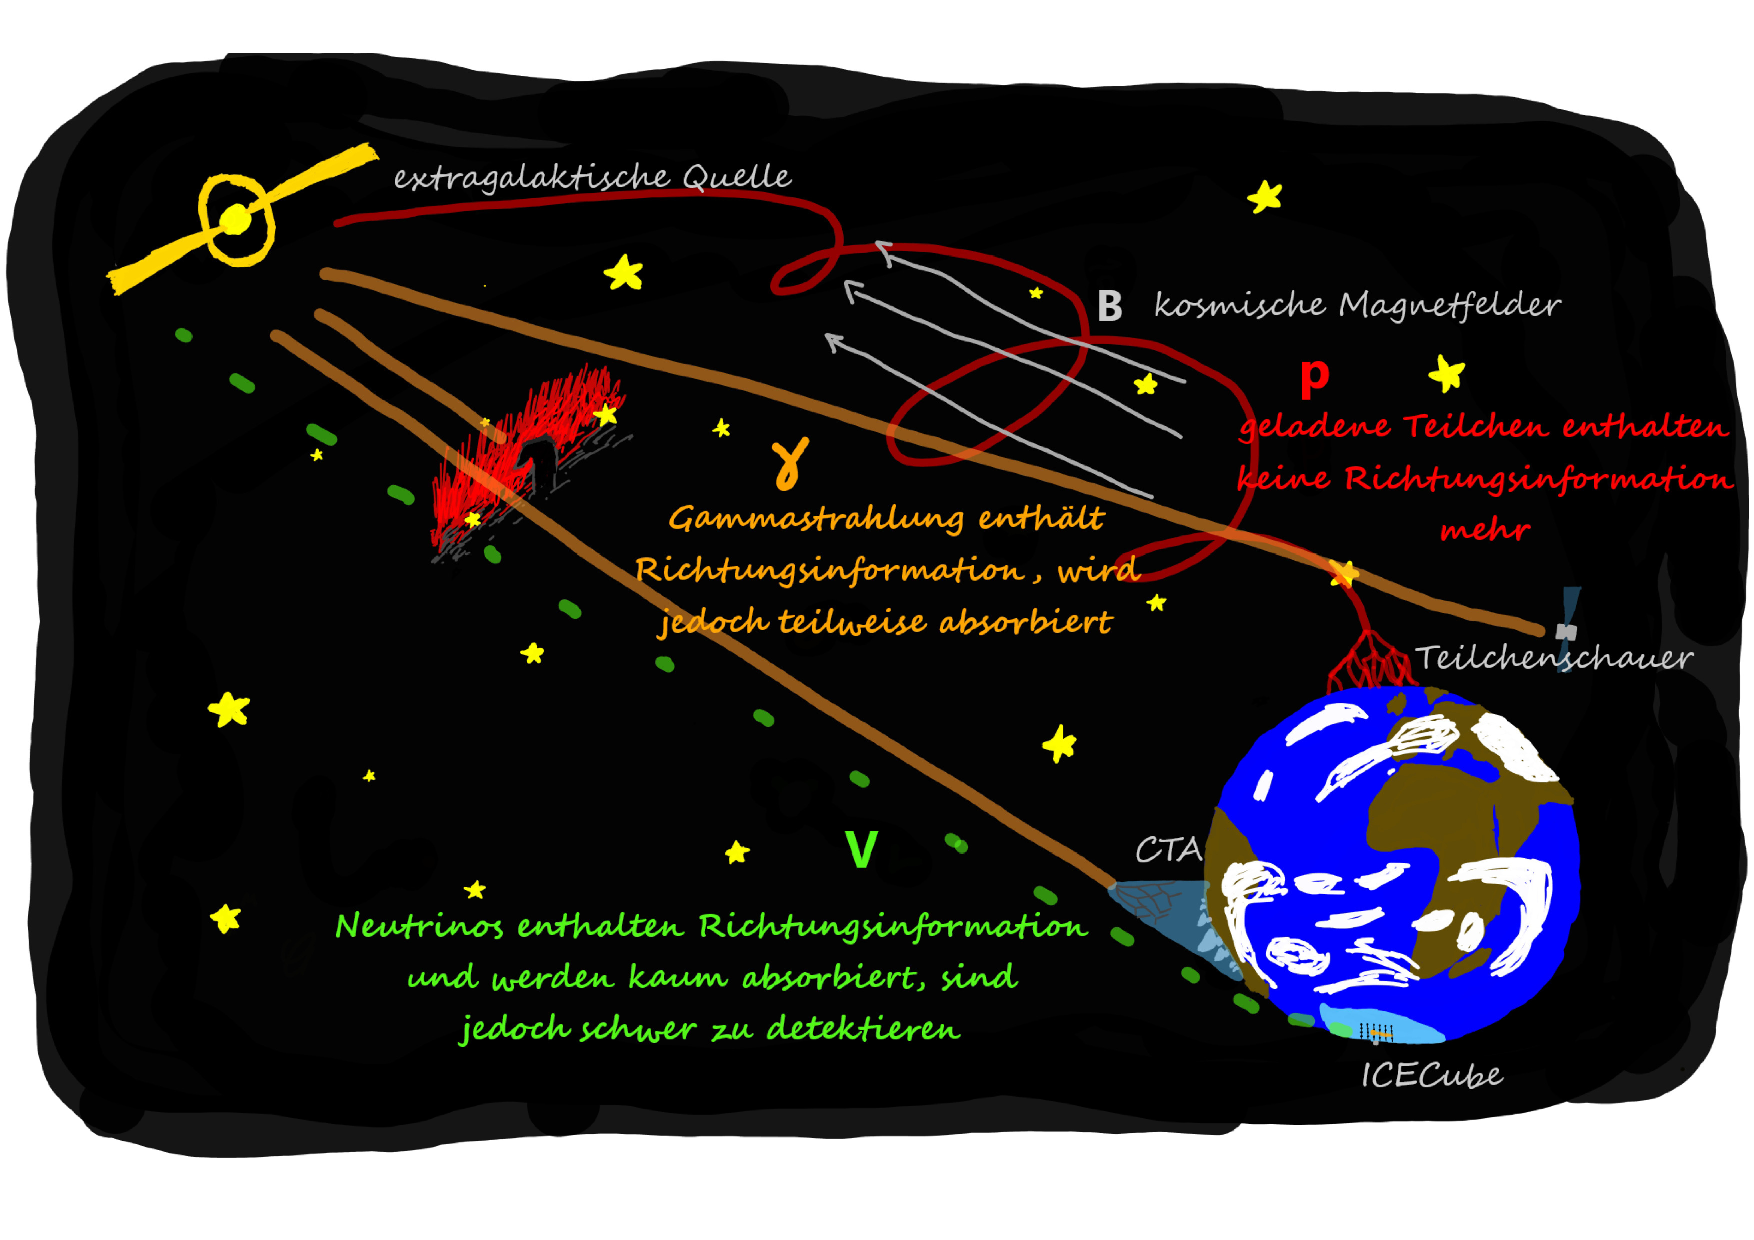
\includegraphics[width=0.7\textwidth]{pictures/Folie5.pdf}
        \caption{}
        \label{abb:folie5}
      \end{figure}
  \end{frame}


  \begin{frame}
    \frametitle{Funtionsweise von CTA}
    \begin{columns}
      \column{0.6\textwidth}
        \begin{figure}
          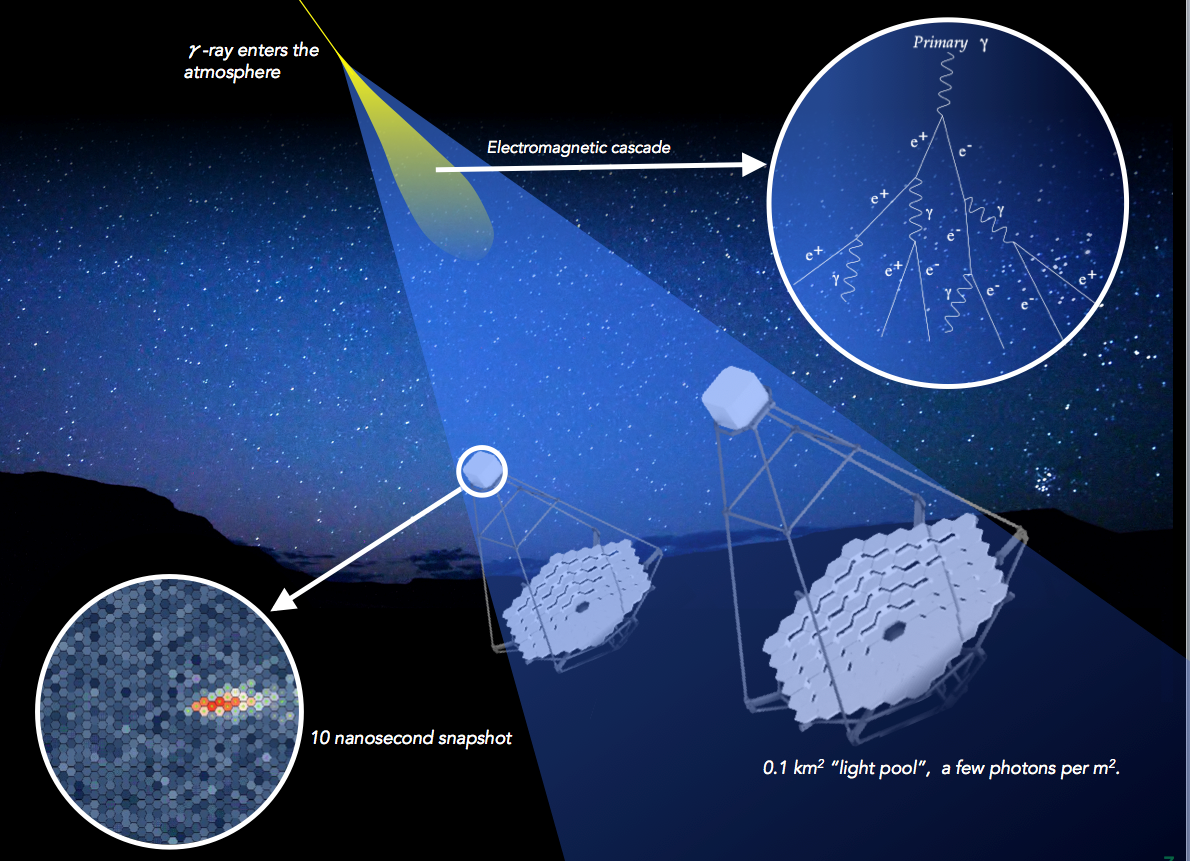
\includegraphics[width=0.95\textwidth]{pictures/CTA.png}
          \caption{CTA hompage (How CTA works)}
          \label{abb:CTA}
        \end{figure}
      \column{0.4\textwidth}
        \begin{itemize}
          \item Photon wechselwirkt mit der Atmosphäre: Schauer entsteht.
          \item Lichtgeschwindigkeit in Atmosphäre $\SI{0.03}{\percent}$ langsamer als Vakuum.
          \item Überlichtschnelle geladene Teilchen senden Kegel aus Cherenkov-Licht aus.
          \item Durchmesser: $\SI{250}{\m}$
          \item Dauer: einige $\si{\nano\s}$.
        \end{itemize}
    \end{columns}
  \end{frame}
  \begin{frame}
    \frametitle{Information über das Schauer}
    \begin{columns}
      \column{0.4\textwidth}
        \begin{itemize}
          \item Hillas Parameter, Wölbung und Krümmung
          \item Scaled Cuts Technik: $SV = \frac{v- \langle v \rangle}{\sigma_v}$ für $v=w\text{;}l$~\cite[104]{SV}
          \item Teleskopart
          \item Anzahl der ausgelösten Teleskope, LST, MST und SST
          \item gesamte Intensität
          \item Art des Primärteilchens
        \end{itemize}
      \column{0.6\textwidth}
        \begin{figure}
          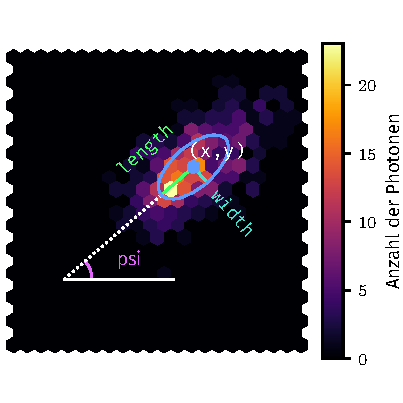
\includegraphics[width=0.7\textwidth]{pictures/hillas_2.pdf}
          \caption{Max Nöthe}
          \label{abb:Hillas}
        \end{figure}
    \end{columns}
  \end{frame}

  \begin{frame}
    \frametitle{Aufgabenspektrum}
    \begin{itemize}
      \item Entdecken neuer galaktischer Gammaquellen (SNR, PWN, Doppelsysteme, galaktische Zentren).
      \item Multiwellenlängen- und Multimessenger-Beobachtungen um hadronische Beschleunigungsprozesse zu untersuchen.
      \item Entdecken neuer Quellen mit großer Rotverschiebung.
      \item Detektieren von Zerfällen der Dunklen Materie.
      \item \dots
    \end{itemize}
  \end{frame}


  \subsection{Maschinelles Lernen}

  \begin{frame}
    \frametitle{Entscheidungsbaum}
    \begin{columns}
      \column{0.7\textwidth}
      \begin{figure}
        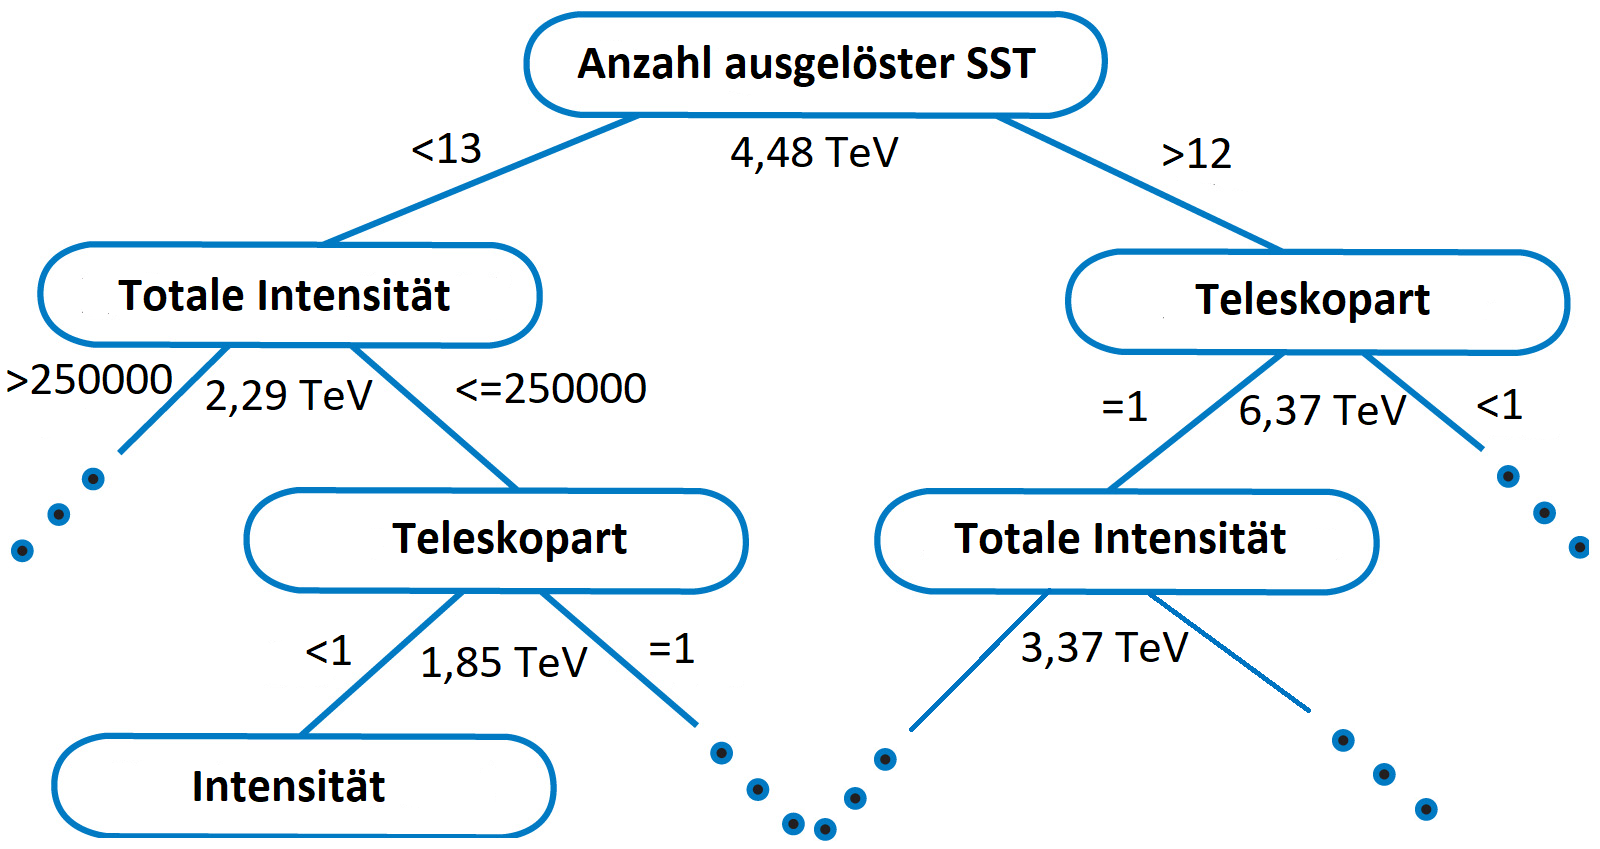
\includegraphics[width=0.8\textwidth]{pictures/Decisiontree.png}
        \caption{}
        \label{abb:DT}
      \end{figure}
      \column{0.3\textwidth}
      \begin{block}{Kriterium}
        \begin{equation*}
          \symbf{H}(\symbf{X}_m) = \frac{1}{N_m}\sum_{i\in N_m}(\symbf{\hat{y}}_i-\symbf{c}_m)^2
        \end{equation*}
        mit
        \begin{equation*}
          \symbf{c}_m = \frac{1}{N_m}\sum_{i\in N_m}\symbf{\hat{y}}_i
        \end{equation*}
      \end{block}
    \end{columns}

  \end{frame}
  \begin{frame}
    \frametitle{Random Forest}
    \begin{columns}
      \column{0.6\textwidth}
      \begin{figure}
        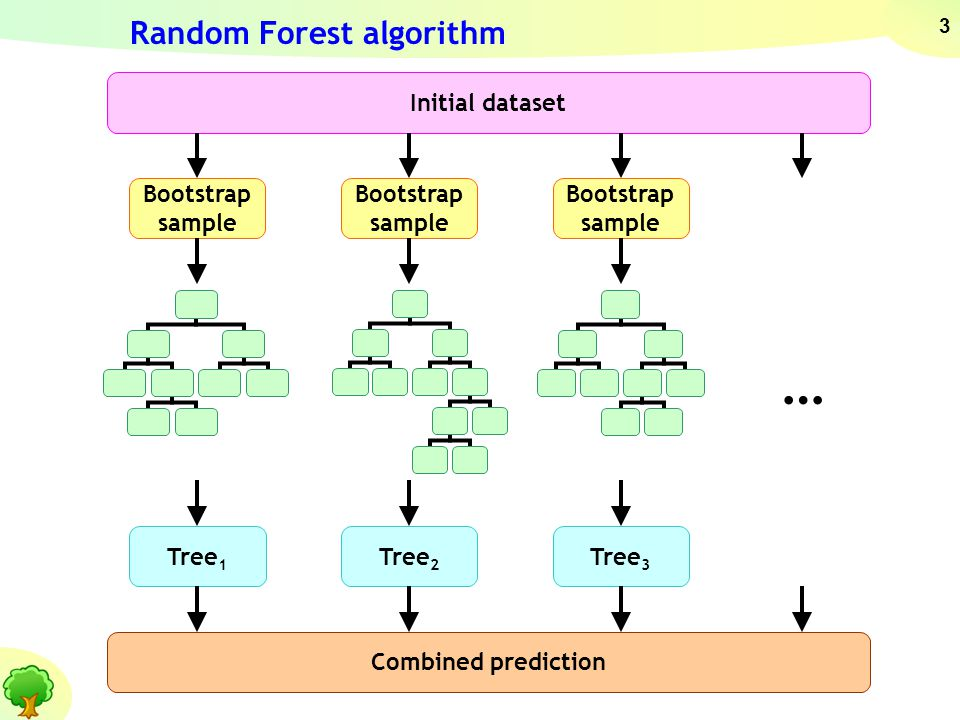
\includegraphics[width=0.9\textwidth]{pictures/RF.jpg}
        \caption{Pavel Polishchuk}
        \label{abb:RF}
      \end{figure}
      \column{0.4\textwidth}
      Warum der Random Forest Algorithmus:
      \begin{itemize}
        \item Interpretierbarkeit
        \item Zeitkomplexität: $\Theta_{\symup{pred}}(M\log(N))$
        \item einfache Datenpräparation
        \item nicht anfällig gegen unbedeutende Attribute
        \item stabiles Ergebnis
      \end{itemize}
    \end{columns}
  \end{frame}

  \section{Ergebnisse}
  \subsection{Rekonstruktion mit RF Regressor}

  \begin{frame}
    \frametitle{Energierekonstruktion mit dem Random Forest}
    \begin{figure}
      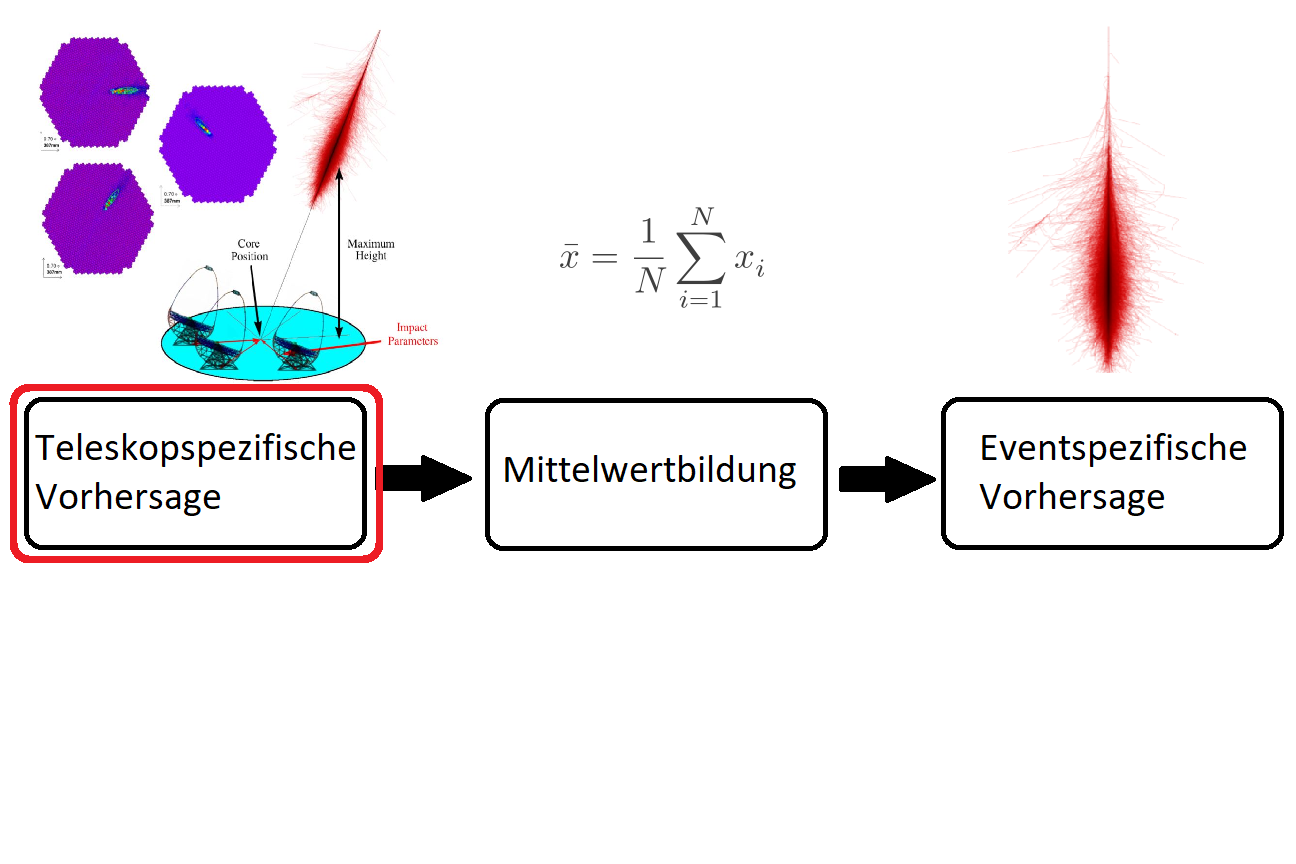
\includegraphics[width=\textwidth]{pictures/Ablauf10.png}
      \caption{}
      \label{}
    \end{figure}
  \end{frame}

  \begin{frame}
    \frametitle{Schätzung jedes Teleskop-Ereignis}
    \begin{columns}
      \column{0.3\textwidth}
          $R^2$-Score:
          \begin{equation*}
            R^2 = 1 - \frac{\sum_i (y_i-\hat{y}_i)^2}{\sum_i (y_i - \overline{y})^2}
          \end{equation*}
      \column{0.7\textwidth}
      \begin{figure}
        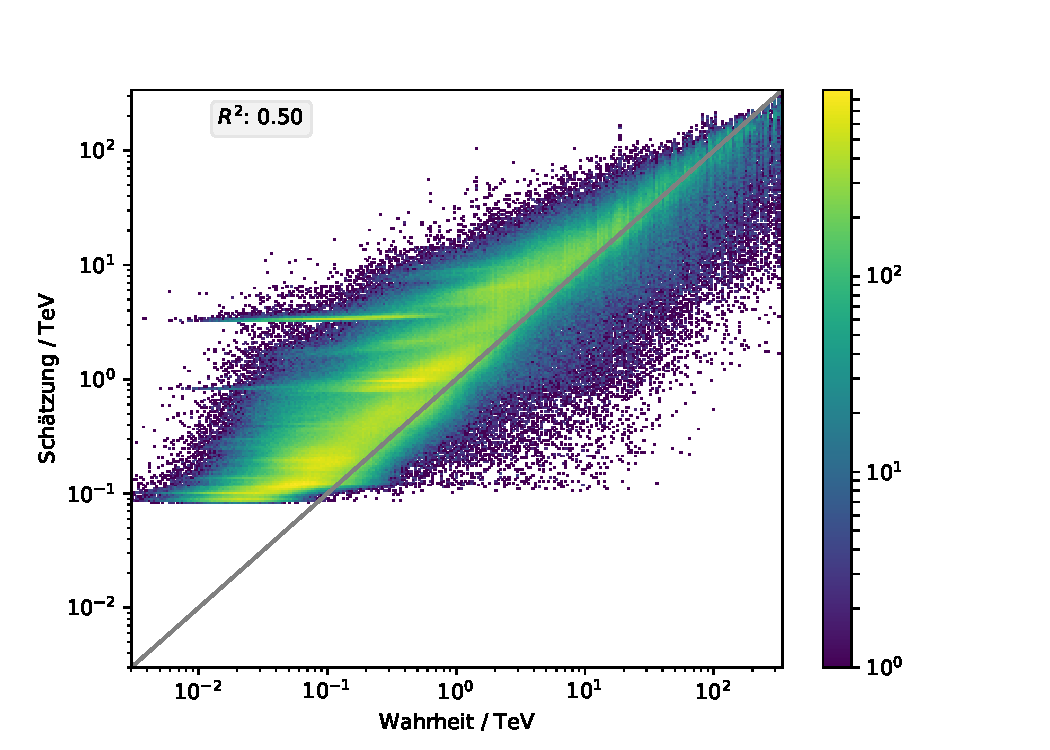
\includegraphics[width=0.9\textwidth]{pictures/RF.pdf}
        \caption{}
        \label{}
      \end{figure}
    \end{columns}
  \end{frame}

  \begin{frame}
    \frametitle{Rangliste der Attribute}
    \begin{columns}
      \column{0.6\textwidth}
      \begin{figure}
        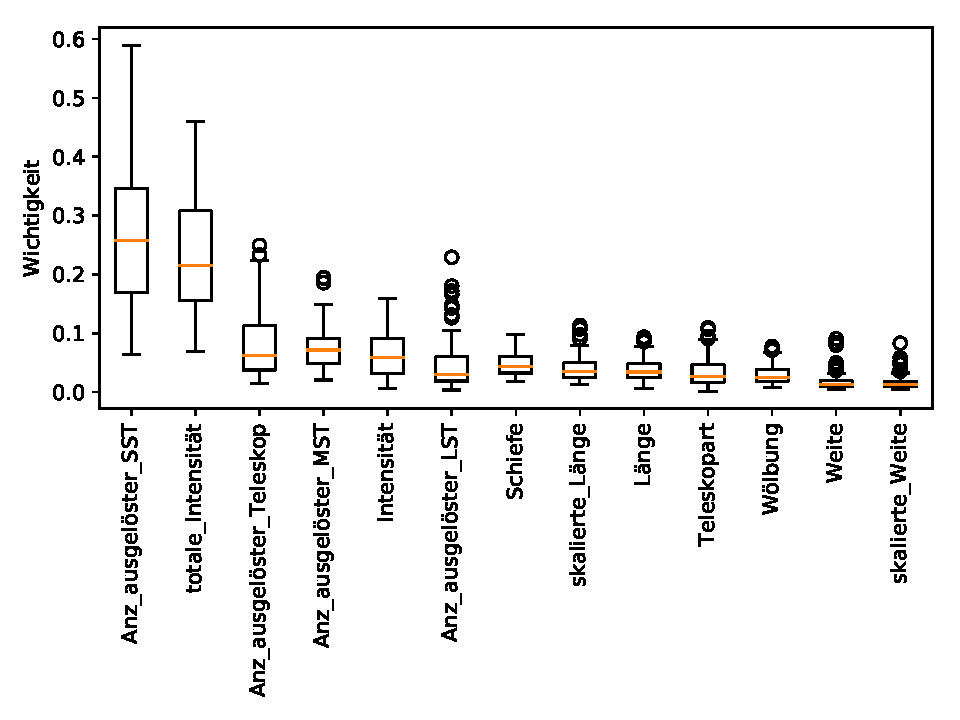
\includegraphics[width=\textwidth]{pictures/feautureimportance_boxplot_firstForest.pdf}
        \caption{}
        \label{}
      \end{figure}
      \column{0.4\textwidth}
      \begin{block}{Kriterium}
        Rangordnung der Attribute in jedem Entscheidungsbaum
      \end{block}
      \begin{itemize}
        \item Aufgrund von Bootstrapping und dem CART-Algorithmus kann eine Verzerrung auftreten.
        \item Attribute mit einer kleinen Anzahl an Kategorien werden unterschätzt.
      \end{itemize}
    \end{columns}
  \end{frame}

  \subsection{Optimierung durch Mittelwert}

  \begin{frame}
    \frametitle{Energierekonstruktion mit dem Random Forest}
    \begin{figure}
      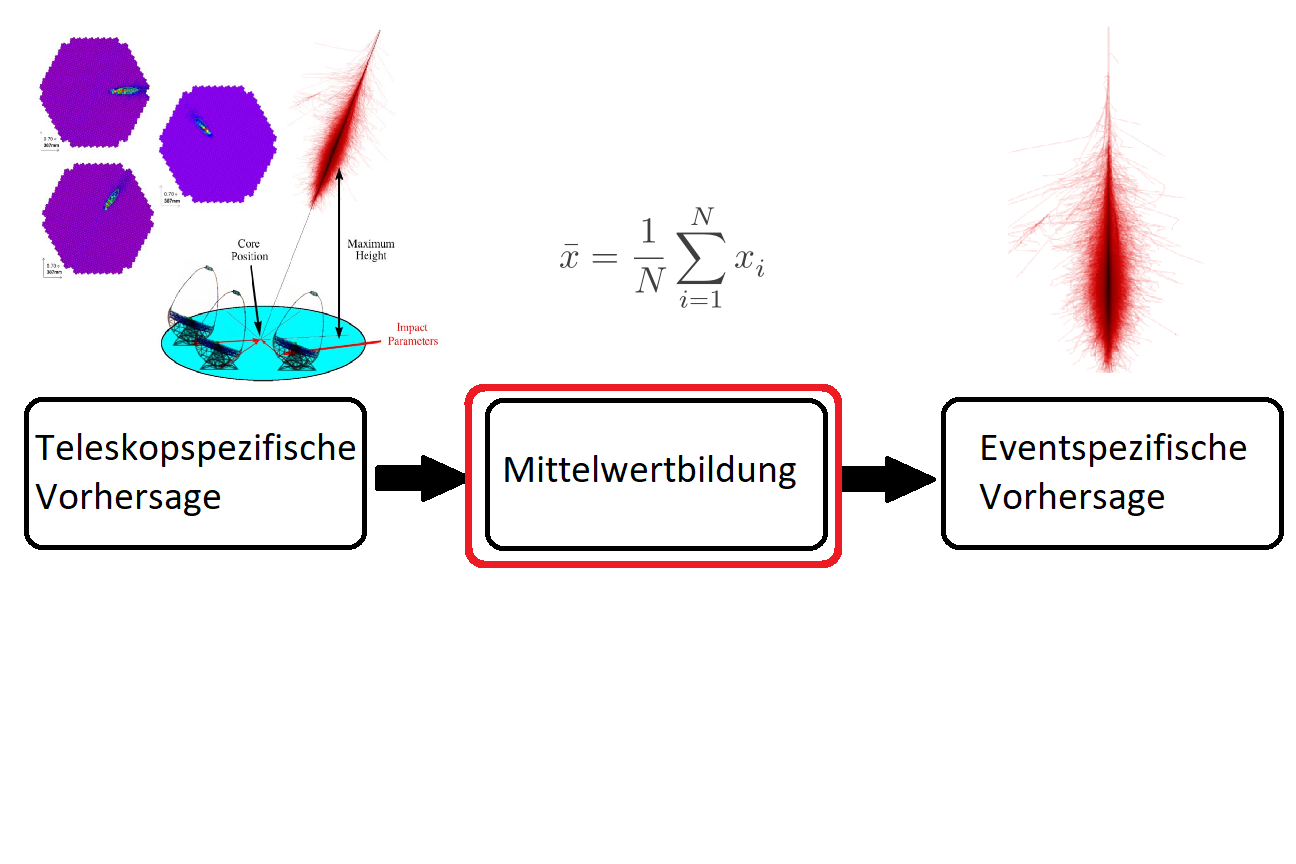
\includegraphics[width=\textwidth]{pictures/Ablauf11.png}
      \caption{}
      \label{}
    \end{figure}
  \end{frame}

  \begin{frame}
    \frametitle{Arithmetisches Mittel und Median}
    \begin{columns}
      \column{0.5\textwidth}
      \begin{figure}
        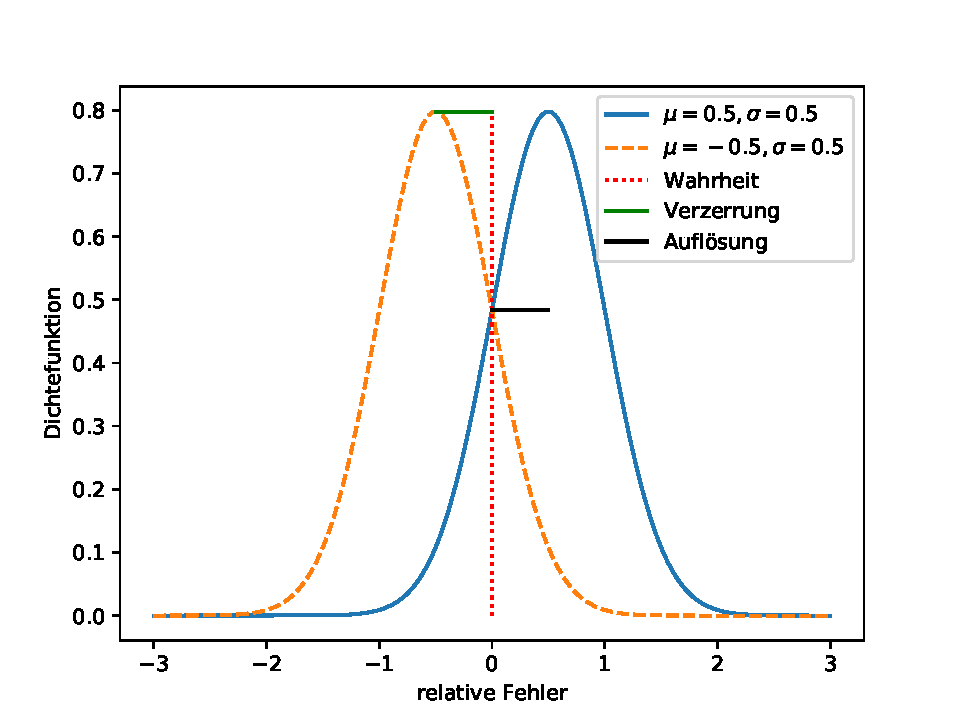
\includegraphics[width=\textwidth]{pictures/Resolution_bias_plot.pdf}
        \caption{}
        \label{}
      \end{figure}
      \column{0.5\textwidth}
      \begin{figure}
        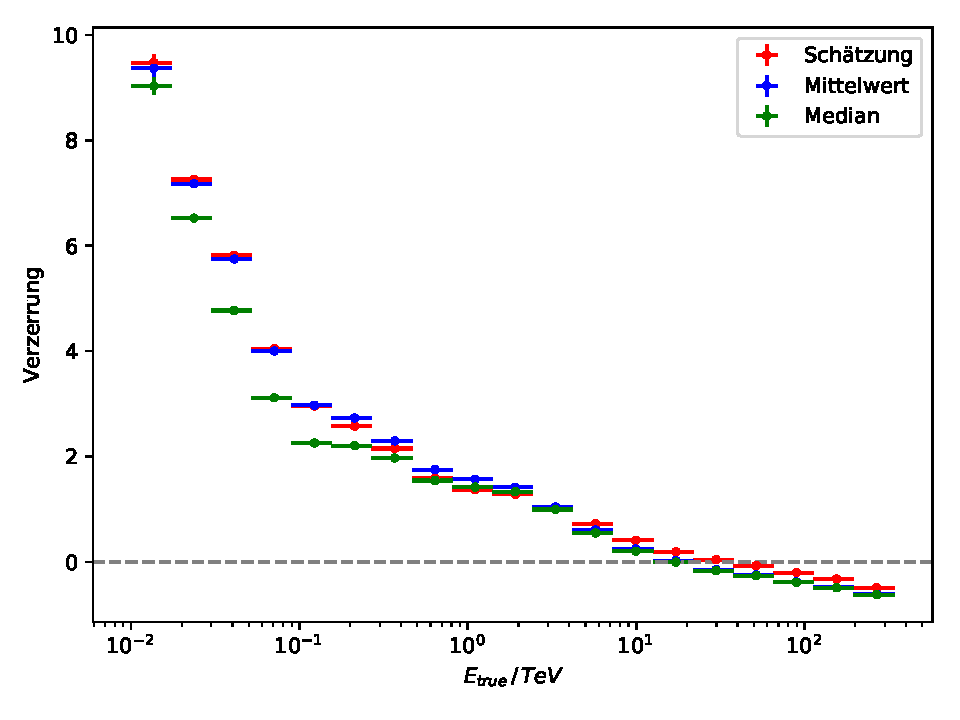
\includegraphics[width=\textwidth]{pictures/RF_mean_bias.pdf}
        \caption{Mittelwert des relativen Fehlers für verschiedene Energiebereiche.}
        \label{}
      \end{figure}
    \end{columns}
  \end{frame}

  \begin{frame}
    \begin{figure}
      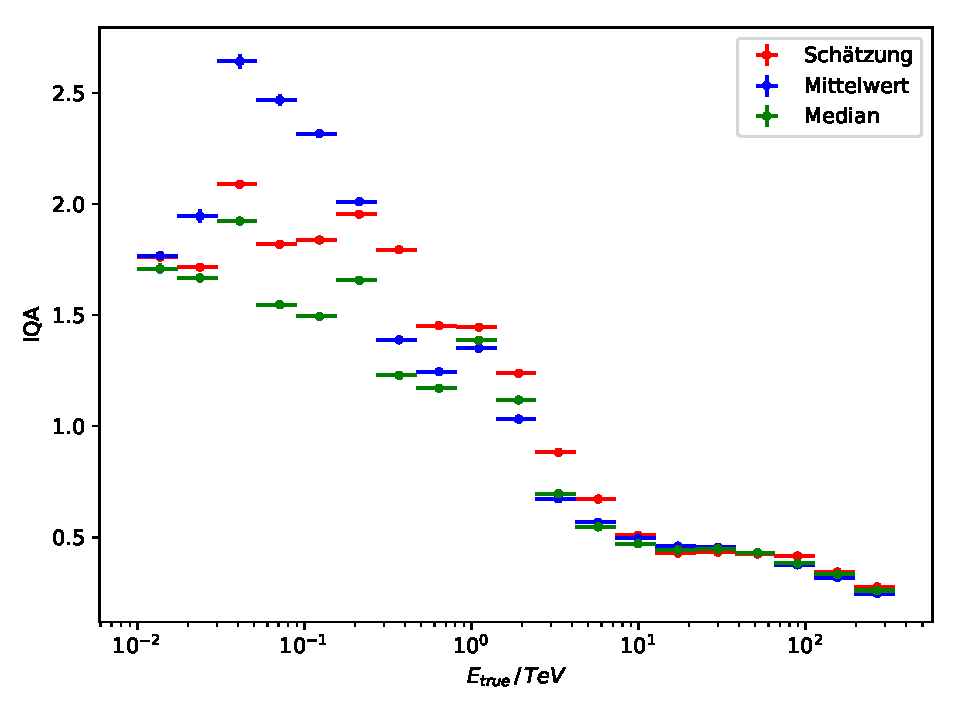
\includegraphics[width=0.5\textwidth]{pictures/RF_mean_resolution.pdf}
      \caption{Die Hälfte des IQA von $\SI{68,26}{\percent}$ des relativen Fehlers für verschiedene Energiebereiche.}
      \label{}
    \end{figure}
  \end{frame}

  \begin{frame}
    \begin{columns}
      \column{0.5\textwidth}
      \begin{figure}
        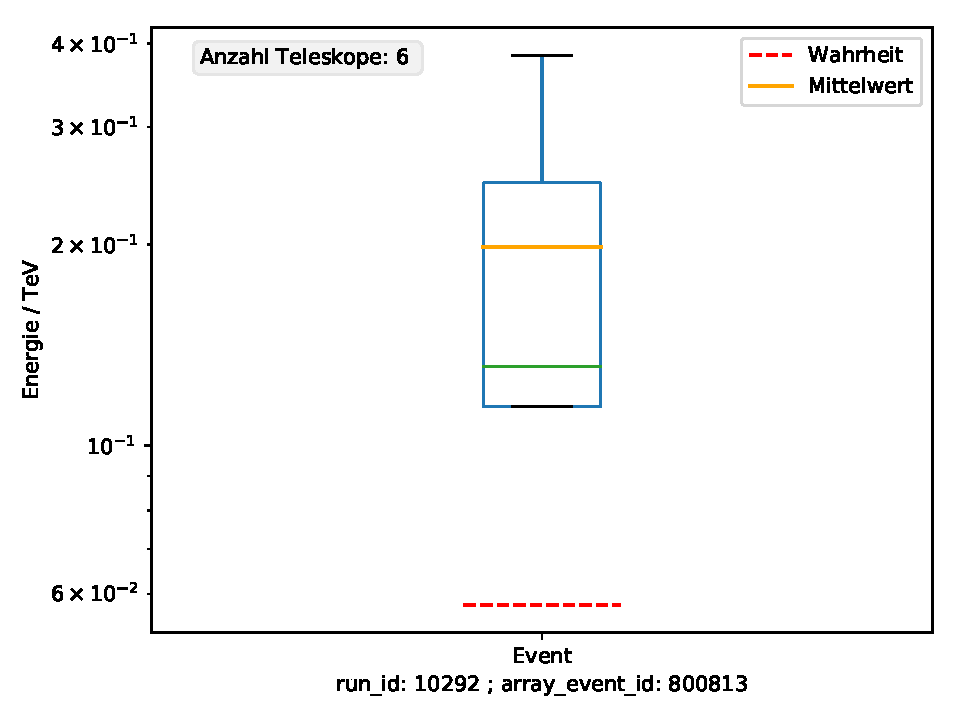
\includegraphics[width=\textwidth]{pictures/pred2.pdf}
        \caption{}
        \label{}
      \end{figure}
      \column{0.5\textwidth}
      \begin{figure}
        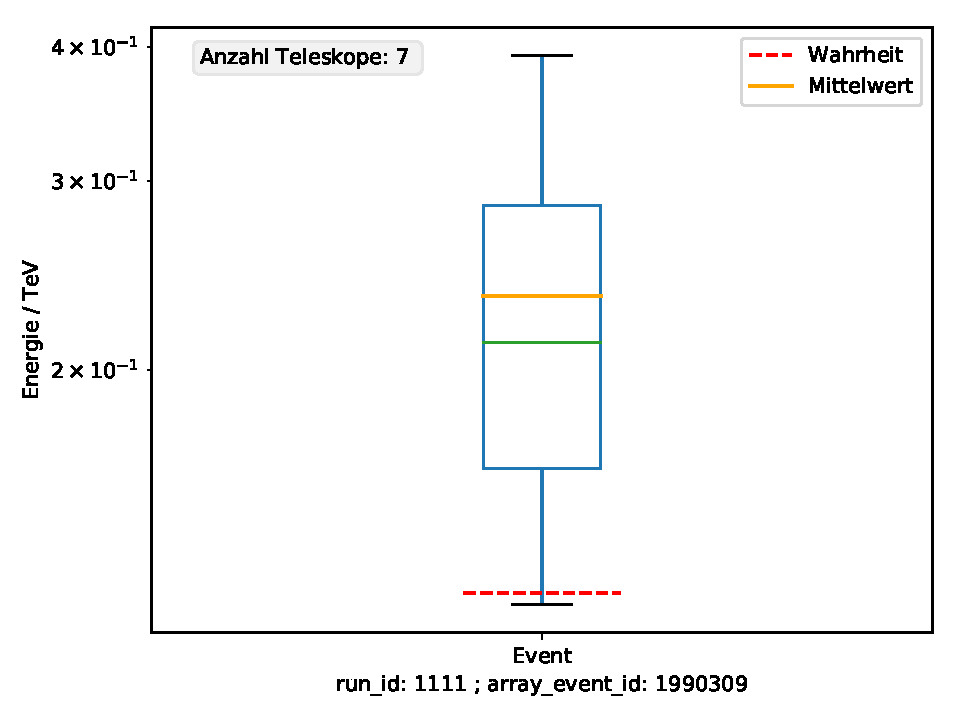
\includegraphics[width=\textwidth]{pictures/pred3.pdf}
        \caption{}
        \label{}
      \end{figure}
    \end{columns}
  \end{frame}

  \begin{frame}
    \frametitle{Intensität als Gewicht}
    \begin{figure}
      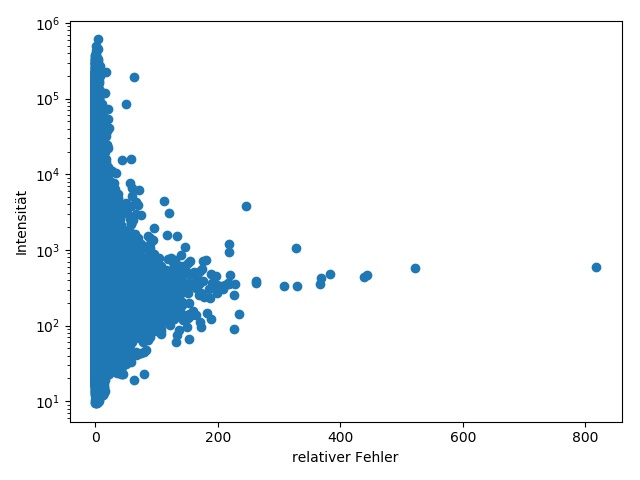
\includegraphics[width=0.5\textwidth]{pictures/intensity.jpg}
      \caption{}
      \label{}
    \end{figure}
  \end{frame}

  \begin{frame}
    \frametitle{Sensitivität als Gewicht}
    \begin{figure}
      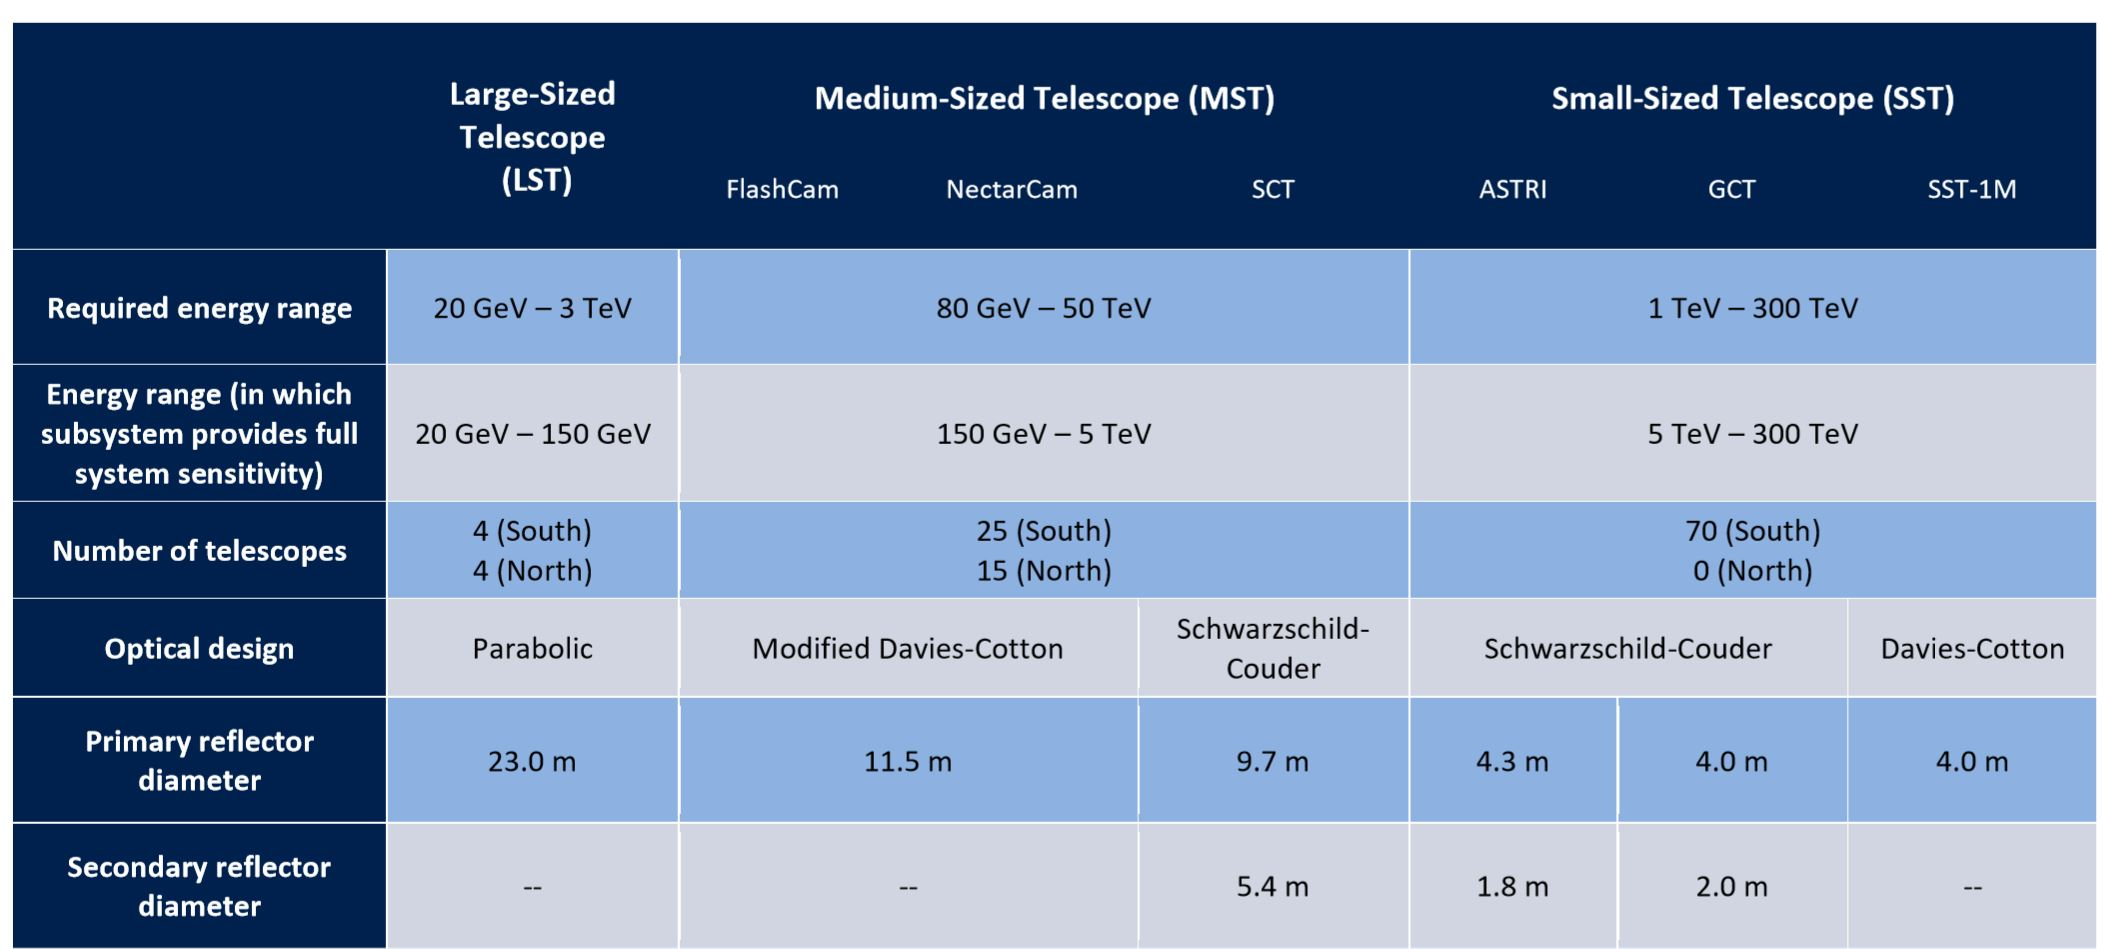
\includegraphics[width=0.7\textwidth]{pictures/Spec.JPG}
      \caption{CTA homepage (CTA technology)}
      \label{}
    \end{figure}
    \begin{columns}
      \column{0.33\textwidth}
      Vollsensitiver Bereich: $\num{2}$
      \column{0.33\textwidth}
      Teilsensitiver Bereich: $\num{1}$
      \column{0.33\textwidth}
       Außerhalb der Bereiche: $\num{0.1}$
    \end{columns}
  \end{frame}

  \begin{frame}
    \begin{columns}
      \column{0.5\textwidth}
      \begin{figure}
        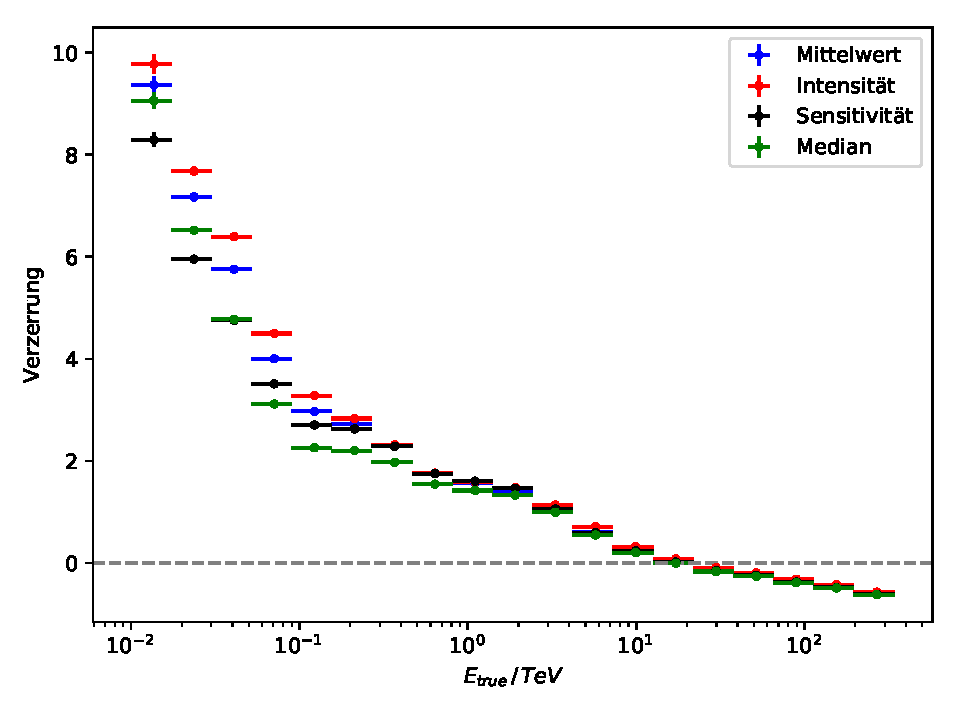
\includegraphics[width=\textwidth]{pictures/RF_weights_bias.pdf}
        \caption{}
        \label{}
      \end{figure}
      \column{0.5\textwidth}
      \begin{figure}
        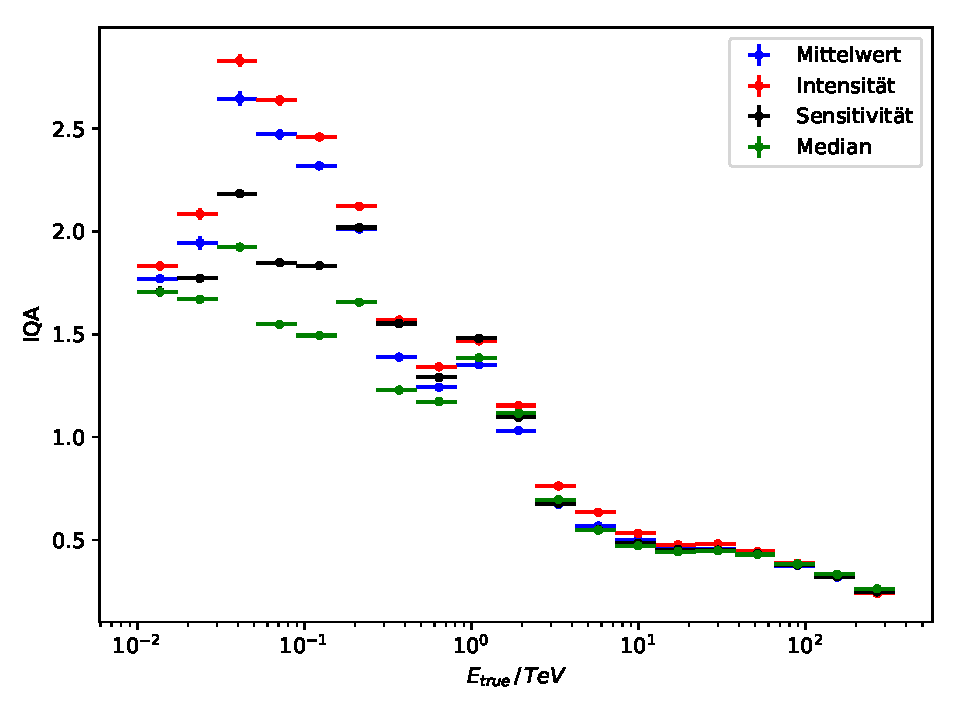
\includegraphics[width=\textwidth]{pictures/RF_weights_resolution.pdf}
        \caption{}
        \label{}
      \end{figure}
    \end{columns}
  \end{frame}

  \subsection{Verschachtelte Methode}

  \begin{frame}
    \frametitle{Energierekonstruktion mit dem Random Forest}
    \begin{figure}
      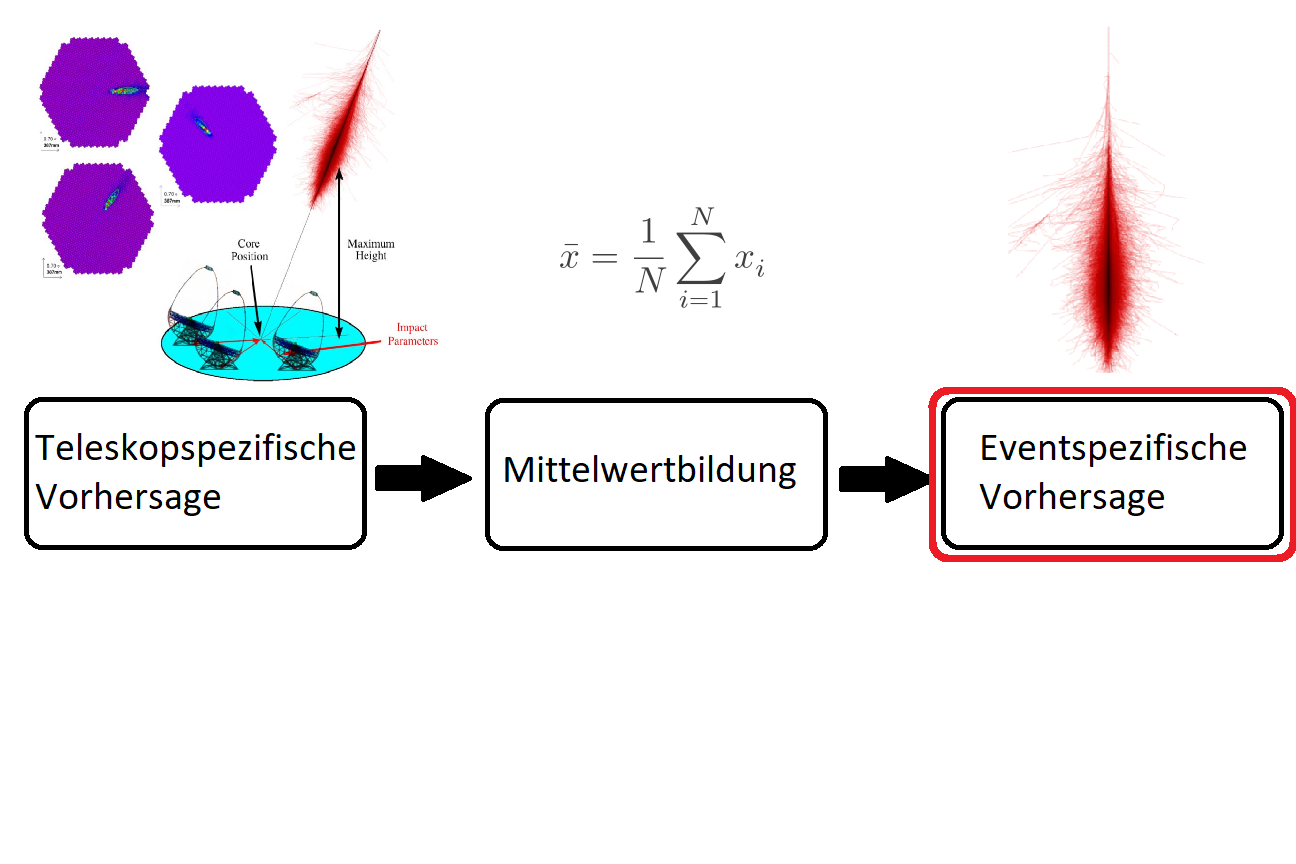
\includegraphics[width=\textwidth]{pictures/Ablauf12.png}
      \caption{}
      \label{}
    \end{figure}
  \end{frame}

  \begin{frame}
    \frametitle{Eventspezifische Vorhersage}
    \begin{columns}
      \column{0.5\textwidth}
      \begin{itemize}
        \item Attribute:
        \begin{itemize}
          \item totale Intensität, Anzahl ausgelöster Teleskope, SST, MST, LST
          \item Mittelwert und Standardabweichung der skalierten Größen
          \item Mittelwert der vorherigen Schätzungen
          \item Mittelwert, Standardabweichung, Maximum und Minimum der Schätzungen der SST, MST und LST
        \end{itemize}
      \end{itemize}
      \column{0.5\textwidth}
      \begin{figure}
        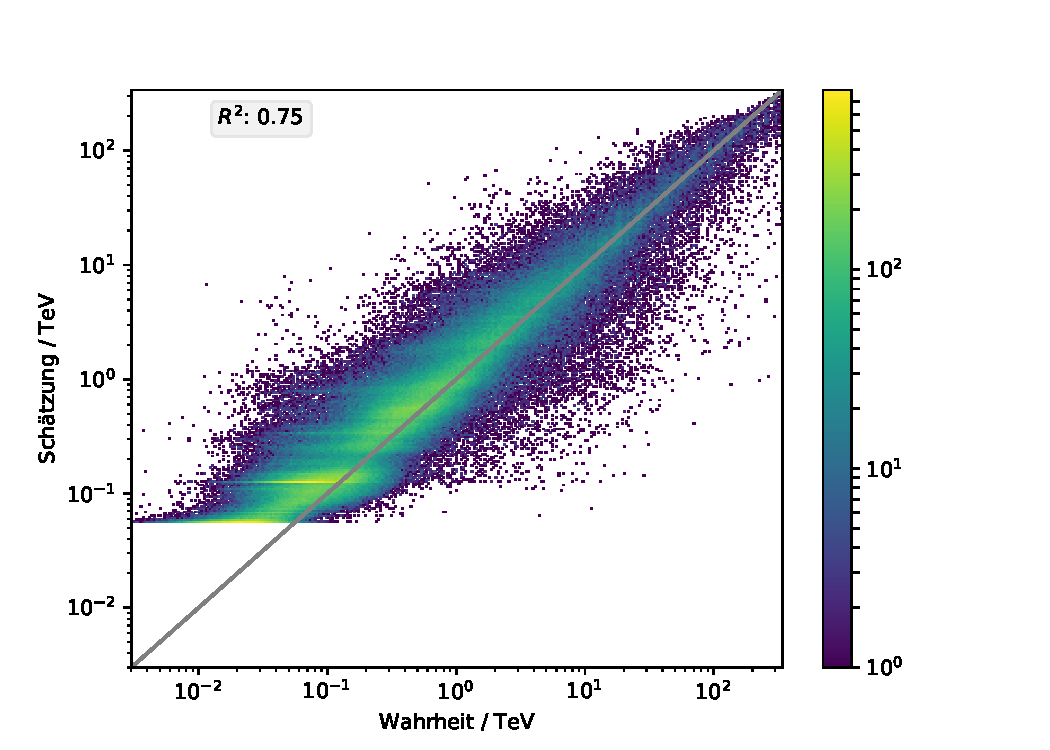
\includegraphics[width=1.1\textwidth]{pictures/RF_encaps.pdf}
        \caption{}
        \label{}
      \end{figure}
    \end{columns}
  \end{frame}

  \begin{frame}
    \frametitle{Rangsliste der Attribute des zweiten Random Forest}
    \begin{figure}
      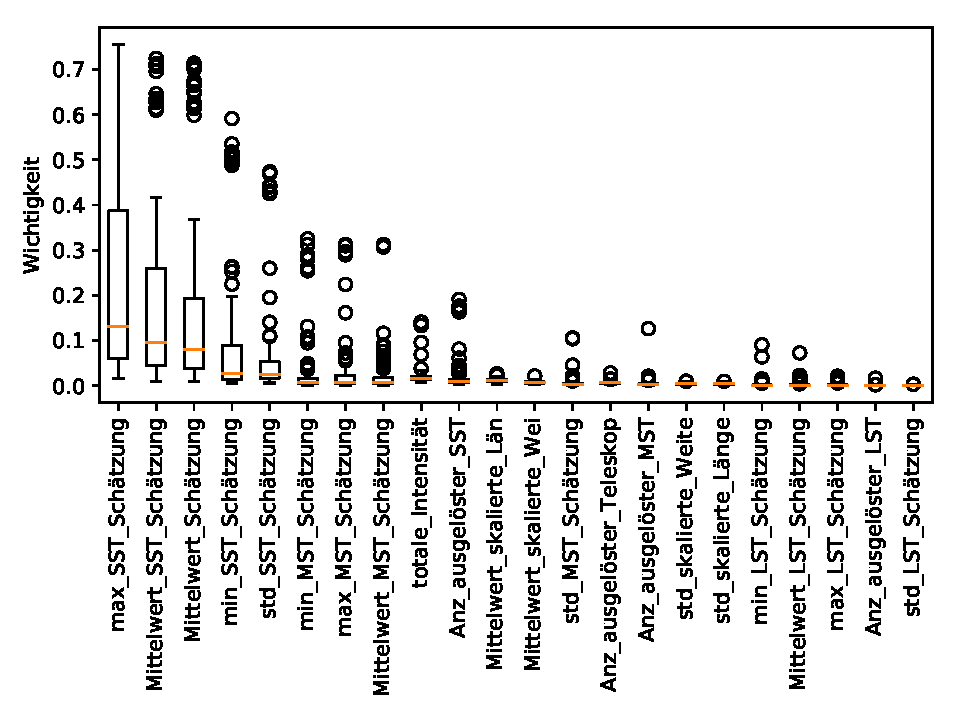
\includegraphics[width=0.55\textwidth]{pictures/feautureimportance_boxplot_secondForest.pdf}
      \caption{}
      \label{}
    \end{figure}
  \end{frame}

  \begin{frame}
    \begin{columns}
      \column{0.5\textwidth}
      \begin{figure}
        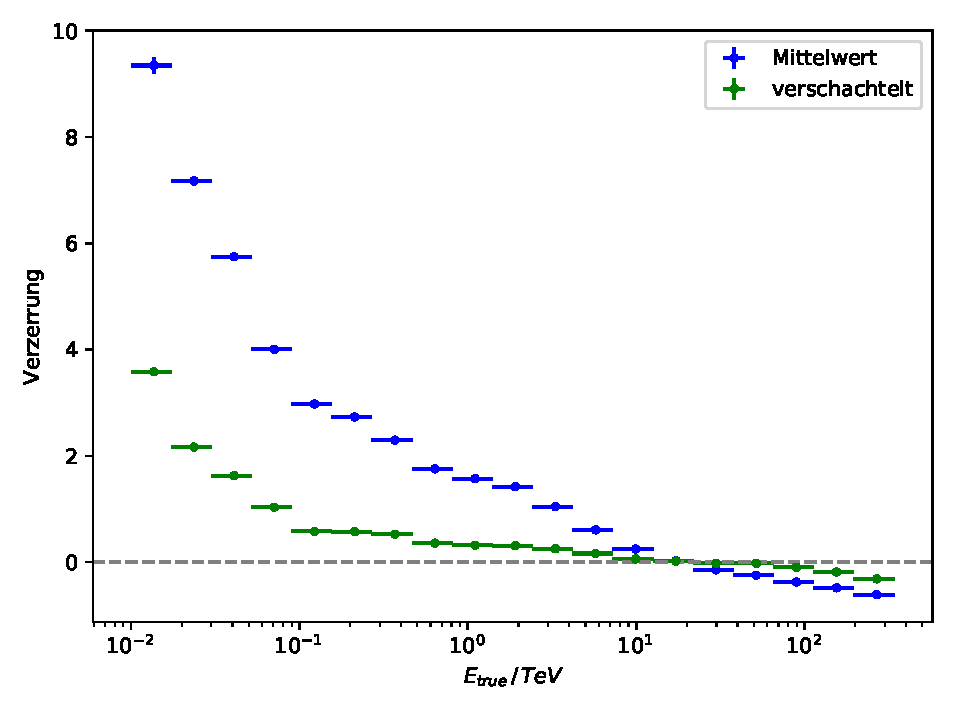
\includegraphics[width=\textwidth]{pictures/RF_nested_bias.pdf}
        \caption{}
        \label{}
      \end{figure}
      \column{0.5\textwidth}
      \begin{figure}
        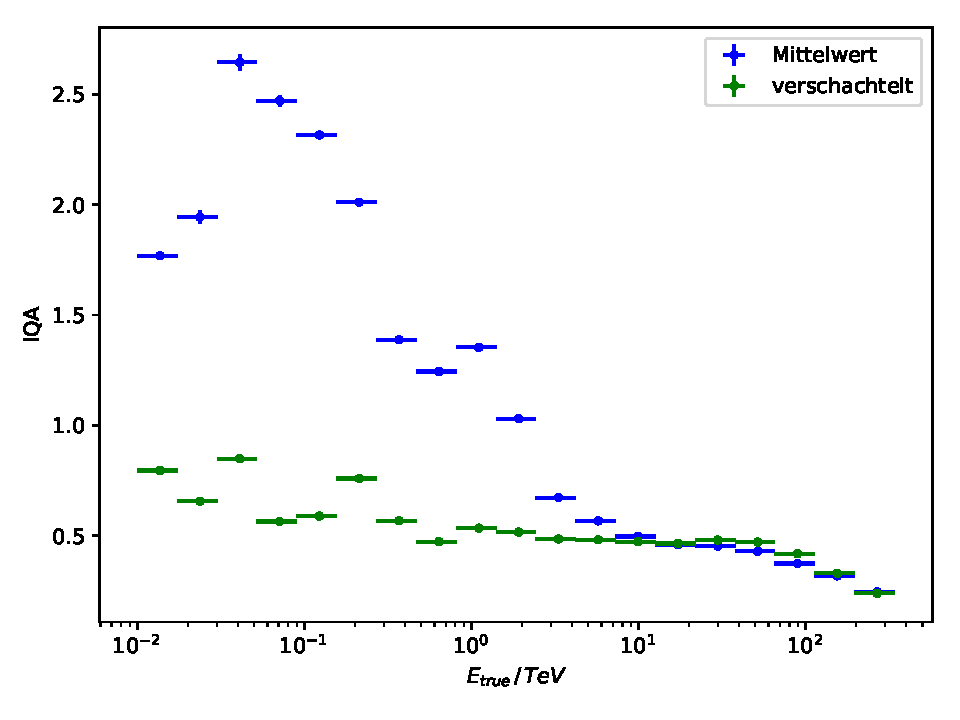
\includegraphics[width=\textwidth]{pictures/RF_nested_resolution.pdf}
        \caption{}
        \label{}
      \end{figure}
    \end{columns}
  \end{frame}

  \subsection{Energie-Transformation}

  \begin{frame}
    \frametitle{Transformation der Energien}
    \begin{figure}
      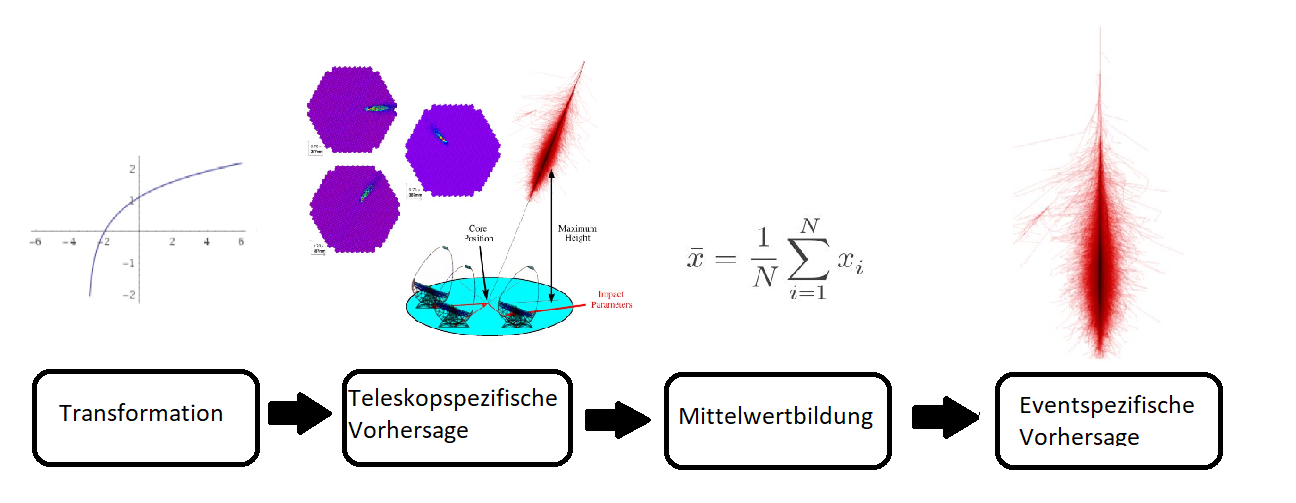
\includegraphics[width=0.6\textwidth]{pictures/Ablauf2.png}
      \caption{}
      \label{}
    \end{figure}
    \begin{columns}
      \column{0.5\textwidth}
      Bijektive Transformation auf $\symbb{R}^+$:
      \begin{equation*}
        E_{\symup{trafo}}=\ln(E_\gamma +3)
        \label{eqn:trafo}
      \end{equation*}
      \column{0.5\textwidth}
      Rücktransformation:
      \begin{equation*}
        E_\gamma = \exp \left(E_{\symup{trafo}}\right)-3
      \end{equation*}
    \end{columns}
  \end{frame}

  \begin{frame}
    \begin{columns}
      \column{0.5\textwidth}
      \begin{figure}
        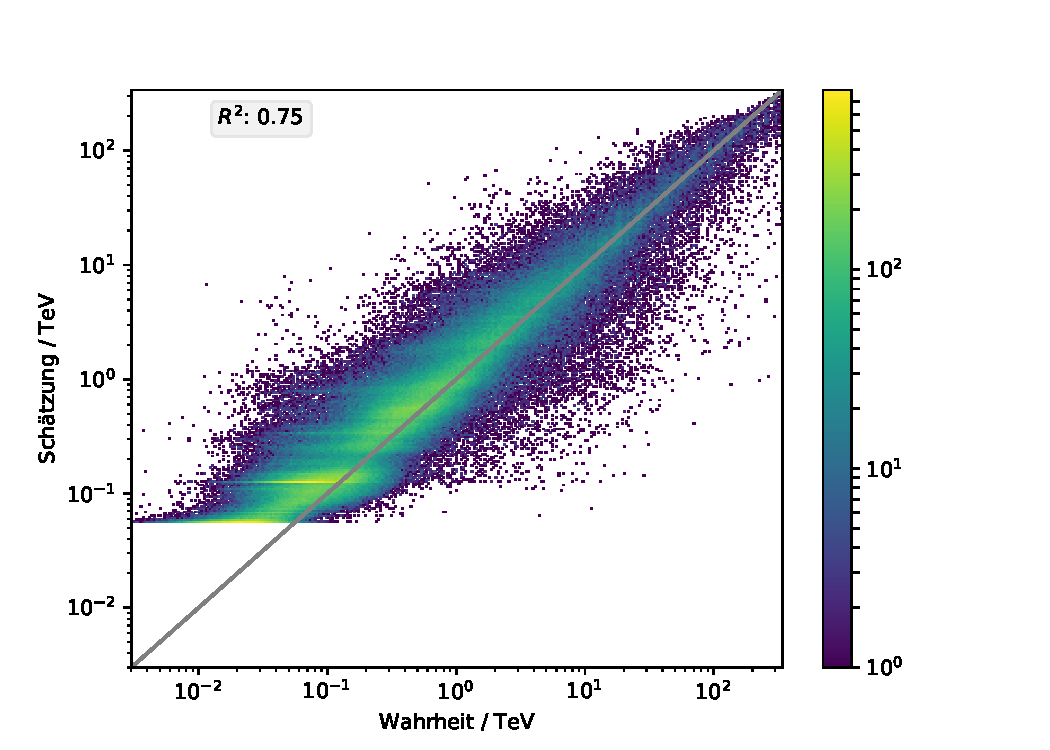
\includegraphics[width=1.1\textwidth]{pictures/RF_encaps.pdf}
        \caption{Ohne Transformation}
        \label{}
      \end{figure}
      \column{0.5\textwidth}
      \begin{figure}
        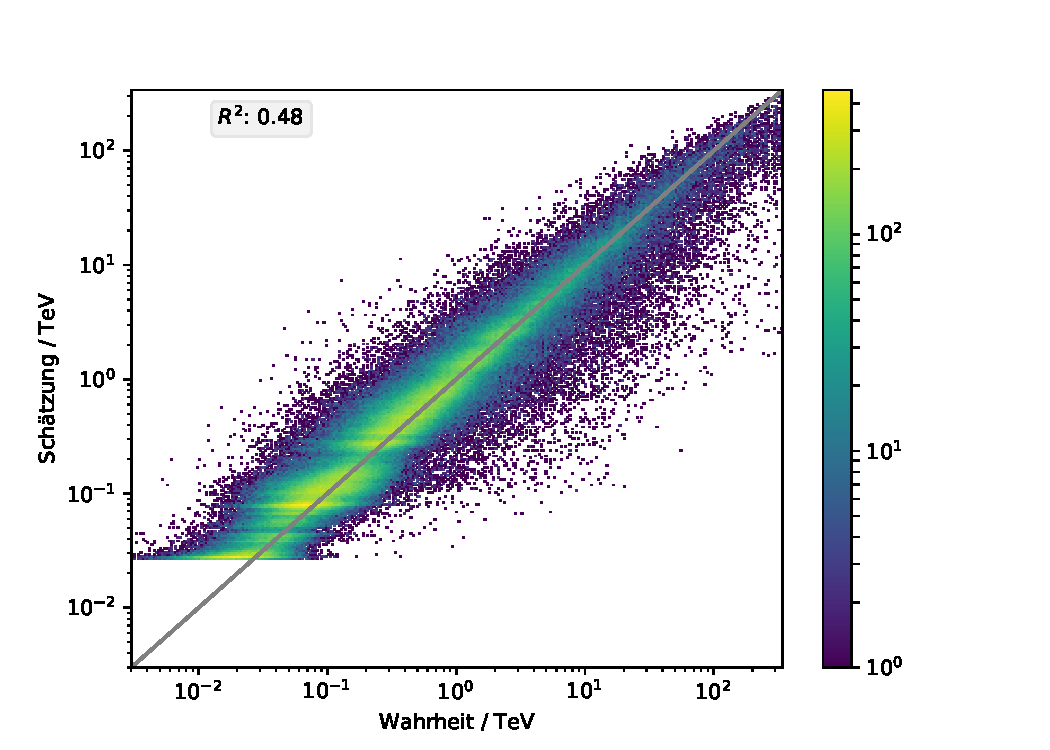
\includegraphics[width=1.1\textwidth]{pictures/trafo_encaps.pdf}
        \caption{Mit Transformation}
        \label{}
      \end{figure}
    \end{columns}
  \end{frame}

  \begin{frame}
    \begin{columns}
      \column{0.5\textwidth}
      \begin{figure}
        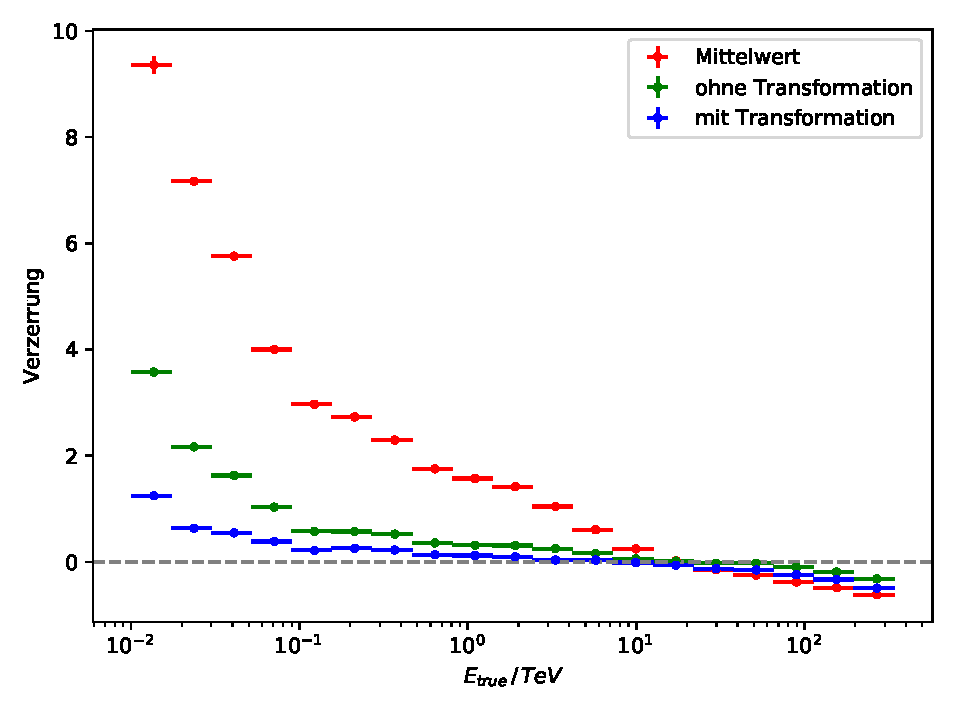
\includegraphics[width=\textwidth]{pictures/trafo_nested_bias.pdf}
        \caption{}
        \label{}
      \end{figure}
      \column{0.5\textwidth}
      \begin{figure}
        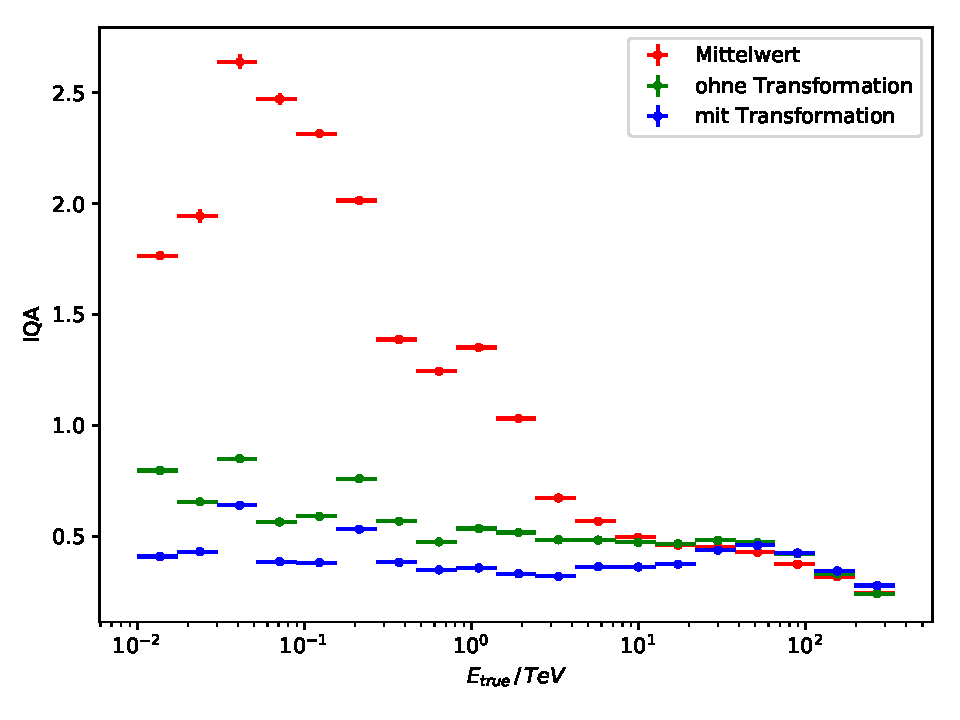
\includegraphics[width=\textwidth]{pictures/trafo_nested_resolution.pdf}
        \caption{}
        \label{}
      \end{figure}
    \end{columns}
  \end{frame}

  \begin{frame}
    \frametitle{Absoluter Fehler}
    \centering
    Mittlere quadratische Fehler:
    \begin{equation*}
      \operatorname{mse} = \frac{1}{N} \sum_i (y_i-\hat{y}_i)^2
    \end{equation*}

    \vspace{0.9cm}

    \begin{tabular}{l|S}
      & $\operatorname{mse}$ \\
      \midrule
      Teleskopspezifische Schätzung & $\SI{102.94}{\tera\eV\squared}$ \\
      Arithmetisches Mittel & $\SI{65.31}{\tera\eV\squared}$ \\
      Median  & $\SI{66.61}{\tera\eV\squared}$ \\
      Gewichtung mit Intensität & $\SI{58.61}{\tera\eV\squared}$ \\
      Gewichtung mit Sensitivität & $\SI{64.72}{\tera\eV\squared}$ \\
      Eventspezifische Schätzung & $\SI{37.18}{\tera\eV\squared}$ \\
      \midrule
      \multicolumn{2}{l}{Transformation:} \\
      \midrule
      Teleskopspezifische Schätzung & $\SI{149.48}{\tera\eV\squared}$ \\
      Arithmetisches Mittel  & $\SI{94.60}{\tera\eV\squared}$ \\
      Eventspezifische Schätzung & $\SI{53.65}{\tera\eV\squared}$ \\
    \end{tabular}
  \end{frame}

  \section{Fazit}

  \subsection{Zusammenfassung}

  \begin{frame}
    \frametitle{Zusammenfassung der Ergebnisse}
    \begin{columns}
      \column{0.5\textwidth}
      \begin{itemize}
        \item Es wurden keine Cuts angewendet.
        \item Anpassung der Methode auf die Aufgabenspezifische Analyse.
        \item Beste Auflösung und geringste Verzerrung des relativen Fehlers bei der verschachtelten Methode mit Transformation
              Es könnte Verzerrung und Auflösung in weiten Bereichen um ca. $\SI{75}{\percent}$ gesenkt werden.
        \item Geringster mittlerer quadratischer Fehler bei der verschachtelten Methode ohne Transformation.
              Der absolute Fehler wurde um ca. $\SI{66}{\percent}$ gesenkt.
      \end{itemize}
      \column{0.5\textwidth}
      \begin{figure}
        \centering
        \parbox{0.49\textwidth}{%
          \subfigure{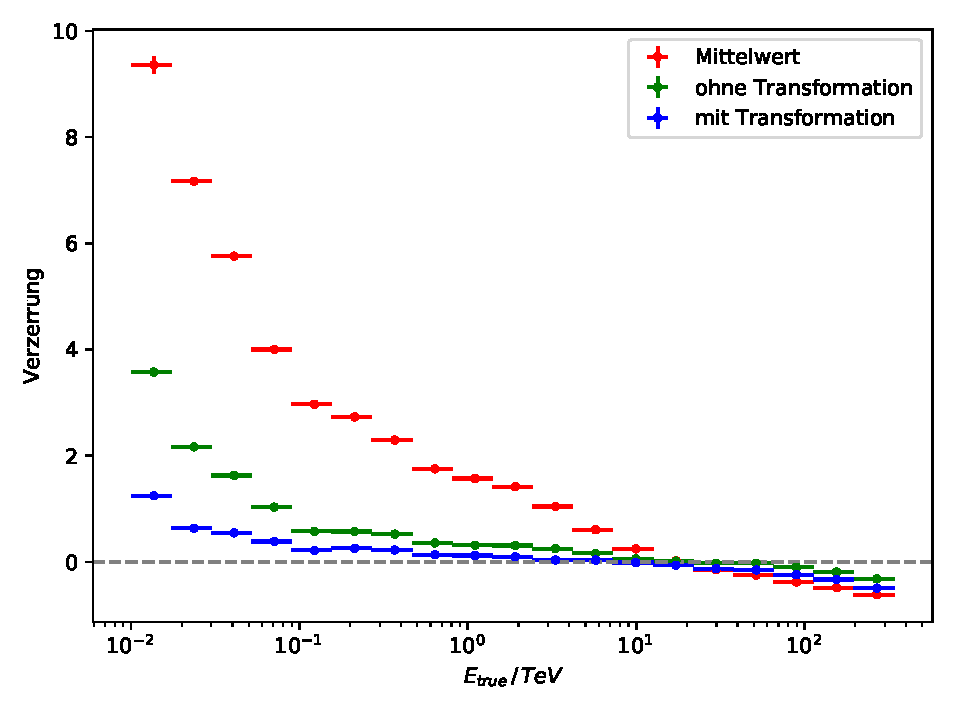
\includegraphics[width=0.55\textwidth]{pictures/trafo_nested_bias.pdf}}

          \subfigure{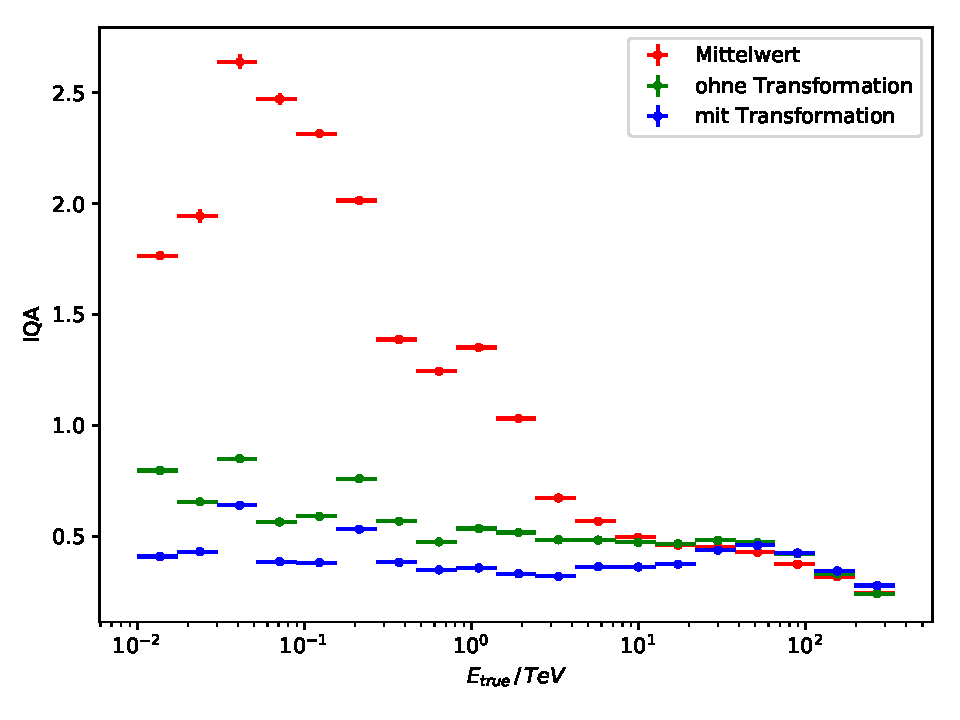
\includegraphics[width=0.55\textwidth]{pictures/trafo_nested_resolution.pdf}}}

      \end{figure}
    \end{columns}
  \end{frame}

  \subsection{Perspektiven}

  \begin{frame}
    \frametitle{Mögliche Perspektiven}
    \begin{columns}
      \column{0.5\textwidth}
      \begin{itemize}
        \item Abstand von Teleskop und Schauer und Höhe des Schauers als Attribut hinzunehmen
        \item aufgabenspezifische Wahl der Transformation
        \item Kriterium für Entscheidungsbaum entwickeln, welches den absoluten Fehler nutzt
      \end{itemize}
      \column{0.25\textwidth}
      \begin{figure}
        
\includegraphics[width=\textwidth]{pictures/sklearn.png}
      \end{figure}
      \begin{figure}
        
\includegraphics[width=\textwidth]{pictures/python.png}
      \end{figure}
      \begin{figure}
        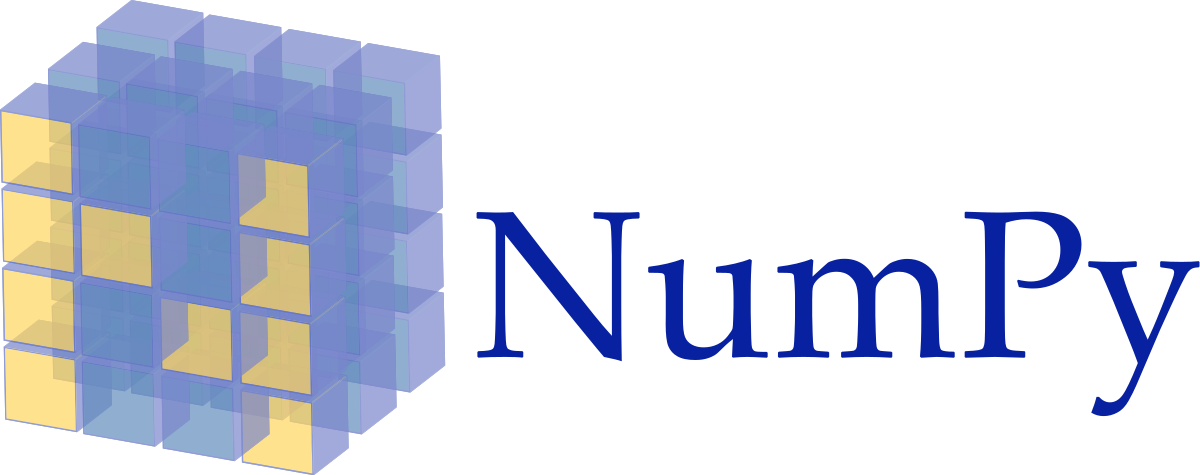
\includegraphics[width=\textwidth]{pictures/numpy.png}
      \end{figure}
      \column{0.25\textwidth}

      \vspace{0.6cm}

      \begin{figure}
        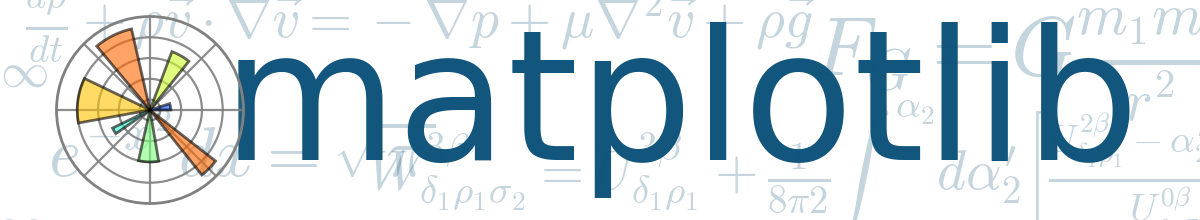
\includegraphics[width=\textwidth]{pictures/matplotlib.png}
      \end{figure}

      \vspace{0.6cm}

      \begin{figure}
        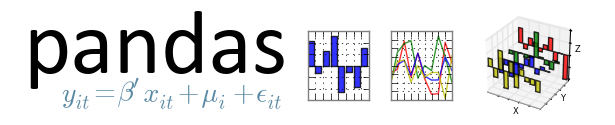
\includegraphics[width=\textwidth]{pictures/pandas.png}
      \end{figure}
    \end{columns}
  \end{frame}

  \section{}

  \begin{frame}
    \printbibliography
  \end{frame}

  \begin{frame}
    \begin{itemize}
      \item Datensatz:
        \begin{itemize}
          \item $\num{3322938}$ Teleskopevents
          \item $\num{996653}$ Arrayevents
          \item $\SI{78}{\percent}$ punktgerichtet und $\SI{22}{\percent}$ diffuse
          \item $\SI{33}{\percent}$ Trainings- und $\SI{66}{\percent}$ Testdatensatz
        \end{itemize}
      \item Random Forest:
        \begin{itemize}
          \item maximale Tiefe $=\num{10}$
          \item Größe des Waldes $=\num{100}$
          \item Anzahl der Attribute $=\sqrt{N}$
          \item minimale Blattgröße $=\num{1}$
        \end{itemize}
    \end{itemize}
  \end{frame}

  \begin{frame}
    \frametitle{Schauer Modell}
    \begin{columns}
      \column{0.5\textwidth}
      Gamma induziertes Schauer:
      \begin{itemize}
        \item $\gamma$
        \item $e^+ ; e^-$
      \end{itemize}
      \column{0.5\textwidth}
      Proton induziertes Schauer
      \begin{itemize}
        \item Hadronische Komponente: Kernfragmente, $\pi$, Kaon, $\dots$
        \item elektromagnetische Komponente: $\gamma$ von $\pi^0$ zerfall
        \item Muonen vom Zerfall der geladenen Mesonen
        \item Neutrios vom Zerfall der geladenen Mesonen und der Muonen
      \end{itemize}
    \end{columns}
    \begin{figure}
      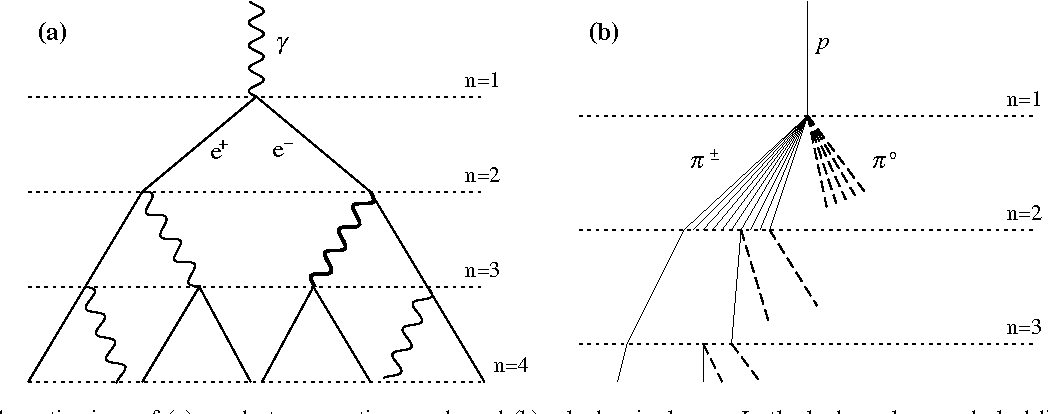
\includegraphics[width=0.7\textwidth]{pictures/Heitler.png}
      \caption{Joseph Matthews}
      \label{}
    \end{figure}
  \end{frame}

  \begin{frame}
    \begin{figure}
      \includegraphics[width=0.5\textwidth]{pictures/CherenkovRadiation.png}
      \caption{wikipedia}
      \label{}
    \end{figure}
  \end{frame}

  \begin{frame}
    \frametitle{Fermi-Beschleunigung}
    \begin{columns}
      \column{0.5\textwidth}
      \textbf{erster Ordnung}
      \begin{equation*}
        \left\langle \frac{\delta E}{E} \right\rangle \approx \frac{2}{3}\frac{\delta v}{c} \text{ ,}
      \end{equation*}
      $\delta v$ Geschwindigkeitsunterschied hinter und vor der Druckwelle
      \begin{figure}
        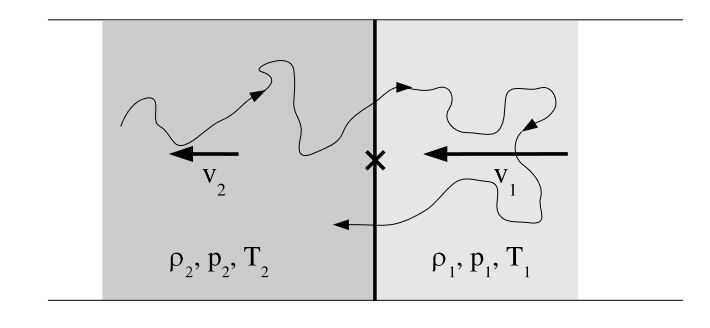
\includegraphics[width=\textwidth]{pictures/firstorderFermi.JPG}
        \caption{Mathieu de Naurois}
        \label{}
      \end{figure}
      \column{0.5\textwidth}
      \textbf{zweiter Ordnung}
      \begin{equation*}
        \left\langle \frac{\delta E}{E} \right\rangle = \frac{8}{2}\left(\frac{v}{c}\right)^2\text{ .}
      \end{equation*}
      $v$ Druckwellengeschwindigkeit
      \begin{figure}
        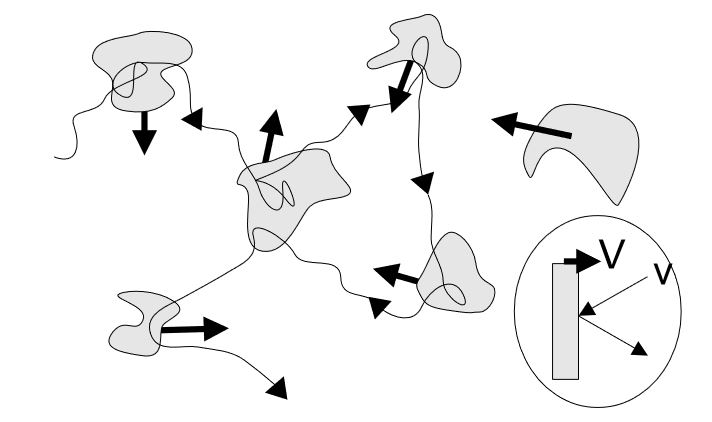
\includegraphics[width=\textwidth]{pictures/secondorderFermi.JPG}
        \caption{Mathieu de Naurois}
        \label{}
      \end{figure}
    \end{columns}
  \end{frame}

  \begin{frame}
    \frametitle{Gammaquellen}
    \begin{columns}
      \column{0.5\textwidth}
      \begin{figure}
        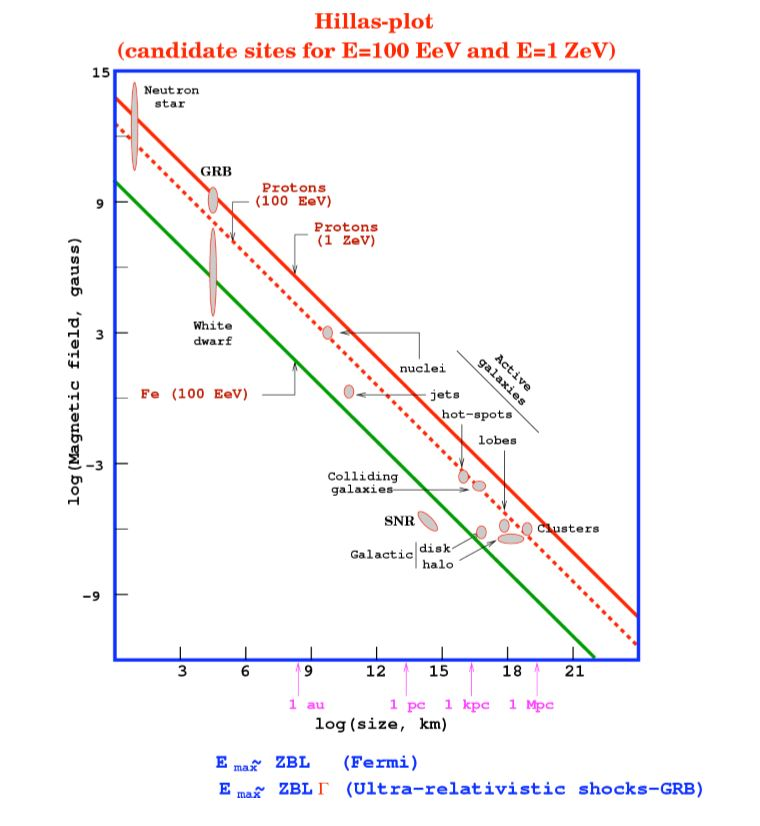
\includegraphics[width=0.9\textwidth]{pictures/gamma_sources.JPG}
        \caption{Mathieu de Naurois}
        \label{}
      \end{figure}
      \column{0.5\textwidth}
      \begin{figure}
        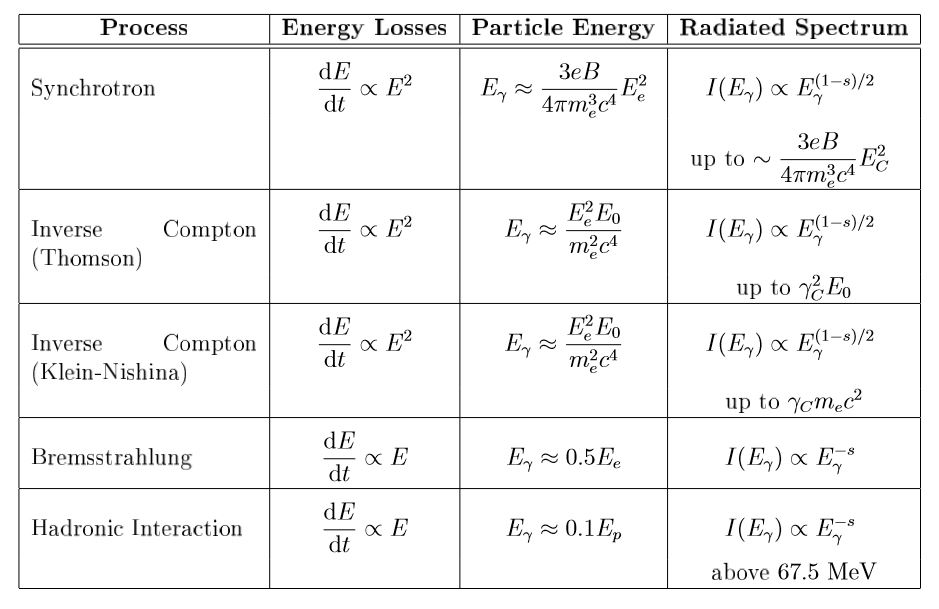
\includegraphics[width=0.9\textwidth]{pictures/gammaprocess.JPG}
        \caption{Mathieu de Naurois}
        \label{}
      \end{figure}
    \end{columns}

  \end{frame}

  \begin{frame}
    \frametitle{Unfolding}
    Aufgrund der endlichen Auflösung ist das Signal
    \begin{equation}
      g(x) = \int_Y R(x|y) \cdot f(y) \symup{d}y
       \text{   oder   } y = A\cdot x \text .
    \end{equation}
    Um das wirkliche Energiespektrum $f$ zu erhalten, muss entfaltet werden.
    Methoden zum Entfalten:
    \begin{itemize}
      \item mit maximum likelihood fit
      \item oder mit Bayes' Theorem
    \end{itemize}
    Bayes' Theorem:
    \begin{equation}
      P(C|E,\Lambda,I) = \frac{P(X|C,\Lambda,I)\cdot P(C|I)}{\sum_C P(E|C,\Lambda ,I)\cdot P(C|I)}
    \end{equation}
    I = informationsstand unter der die Analyse gemacht wurde und
    \begin{equation}
      \lambda_{ij} = P(E_j|C_i,I)
    \end{equation}
    Resolutionmatrix. Mit
    \begin{equation}
      \theta_{ij} = \frac{\lambda_{ij}\cdot P(C_i|I)}{\sum_i \lambda_{ij}\cdot P(C_i|I)} = P(C_i|E_j,I)
    \end{equation}
    lässt sich dann C berechnen
  \end{frame}

  \begin{frame}
    \frametitle{Konvergenz des RF}
    Wenn die Anzahl der Entscheidungsbäume in einem RF erhöht wird, konvergiert der generalisierte Fehler
    \begin{equation}
      PE = P_{X,y}(mg(X,y)<0)
    \end{equation}
    gegen
    \begin{equation}
      P_{X,y}(P_\theta(h(X,\theta)=y)-\max_{j\neq y}P_\theta(h(X,\theta)=j)<0)
    \end{equation}
    und es kann durch eine Vergrößerung des Waldes nicht zum Übertraining kommen.
    \begin{equation}
      mg(X,y) = av_k I(h_k(X)=y) - \max_{j \neq y}av_k I(h_k(X)=j)
    \end{equation}
    die Gewinn-Funktion, $h_k(X)$ = Vorhersage des $k$-ten Entscheidungsbaumes; $I(\cdot)$ die charakteristische Funktion;
    $mg(X,y) > 0$ -> richtiges Ergebnis des RF; $\theta$ = für den Entscheidungsbaum gewählte Attribute.
  \end{frame}

\end{document}
